%
% File:     example.tex
%
% Document based on the template for thesis and dissertations
% developed by Steven White and Malcolm Hutson.
%
% Extensively modified by Adam Lewis (awlewis@cacs.louisiana.edu) to
% meet the UL Graduate School requirements as of Spring 2011. 
%
% Unless otherwise expressly stated, this work is licensed under the
% Creative Commons Attribution-Noncommercial 3.0 United States License. To
% view a copy of this license, visit
% http://creativecommons.org/licenses/by-nc/3.0/us/ or send a letter to
% Creative Commons, 171 Second Street, Suite 300, San Francisco,
% California, 94105, USA.
%
% THE SOFTWARE IS PROVIDED "AS IS", WITHOUT WARRANTY OF ANY KIND, EXPRESS
% OR IMPLIED, INCLUDING BUT NOT LIMITED TO THE WARRANTIES OF
% MERCHANTABILITY, FITNESS FOR A PARTICULAR PURPOSE AND NONINFRINGEMENT.
% IN NO EVENT SHALL THE AUTHORS OR COPYRIGHT HOLDERS BE LIABLE FOR ANY
% CLAIM, DAMAGES OR OTHER LIABILITY, WHETHER IN AN ACTION OF CONTRACT,
% TORT OR OTHERWISE, ARISING FROM, OUT OF OR IN CONNECTION WITH THE
% SOFTWARE OR THE USE OR OTHER DEALINGS IN THE SOFTWARE.

\documentclass[12pt]{report}	% The documentclass must be ``report''.

% Dissertation package style file.
\usepackage{template/uldiss}  		

% 
% Here is a collection of optional packages that can make your life
% far more pleasant while writing your thesis, prospectus, or
% dissertation.   You should tailor these to match the specific needs
% for your document.
%
\usepackage{amsmath,amsthm,amsfonts,amscd,amssymb} % Some packages to write mathematics.
\usepackage{eucal} % Euler fonts
\usepackage{verbatim} % Allows quoting source with commands.
% The listings package supports the pretty-printing of source code.
% The listings packages supports the most commonly used programming
% languages.
\usepackage{listings}
\lstloadlanguages{Matlab,C++,C,Pascal}
\lstset{
         basicstyle=\footnotesize\ttfamily, 
         %numbers=left,              
         numberstyle=\tiny,          
         %stepnumber=2,              
         numbersep=5pt,              
         tabsize=2,                  
         extendedchars=true,         
         breaklines=true,            
         keywordstyle=textbf,    
         stringstyle=\ttfamily, 
         showspaces=false,       
         showtabs=false,         
         xleftmargin=17pt,
         framexleftmargin=17pt,
         framexrightmargin=5pt,
         framexbottommargin=4pt,
         %backgroundcolor=\color{lightgray},
         showstringspaces=false  
 }
% The caption package is used for fancy formatting of figure, table, and
% other captions.  It is very useful when combined with the listings package.
\usepackage{caption}
\DeclareCaptionFont{white}{\color{white}}
\DeclareCaptionFormat{listing}{\colorbox[cmyk]{0.43, 0.35, 0.35,0.01}{\parbox{\textwidth}{\hspace{15pt}#1#2#3}}}
\captionsetup[lstlisting]{format=listing,labelfont=white,textfont=white, singlelinecheck=false, margin=0pt, font={bf,footnotesize}}
\usepackage{pdfpages}
%
% The graphicx package is the standard package for importing of graphics
% into LaTeX documents.   Note that we configure the package to, by
% default, look for PNG, JPEG, and PDF files in a sub-directory of the
% current directory.
\usepackage{graphicx}
\DeclareGraphicsExtensions{.png,.jpg,.pdf}
\graphicspath{{graphics/}}
%
% Use the subfig package for dealing with multiple part figures.
%\usepackage[caption=false,labelfont=sf,textfont=sf,captionskip=5pt]{subfig}
% 
% The comment package is useful when you use EMACS for editing LaTeX
% documents.  The table editor in EMACS orgtbl-mode interfaces with this
% package for easy editing of tables using the org-mode table editing
% functions. 
\usepackage{comment}

%% imported packages
%%
\usepackage{xargs}

\usepackage{mathpartir}
\usepackage{mathtools}
\usepackage{lambda,cc}
\usepackage[noshare]{vlc}
\usepackage{hyperref}
\usepackage{xcolor}
\usepackage{calc}
\usepackage[labelformat=simple]{subcaption}
\captionsetup{compatibility=false}
\renewcommand\thesubfigure{(\alph{subfigure})}

\usepackage{stmaryrd}
\setcounter{tocdepth}{3}
\usepackage{makecell}
%\usepackage{setspace}

\usepackage[inline]{enumitem}
\usepackage{epstopdf}
\usepackage{booktabs}

\newcommand{\pg}{\ensuremath{p}}
\newcommand{\pgi}{\ensuremath{\pg_i}}
\newcommand{\pgj}{\ensuremath{\pg_j}}
\newcommand{\pgk}{\ensuremath{\pg_k}}

\newcommand{\seqijk}{\ensuremath{\dots,\pgi,\dots,\pgj,\dots,\pgk,\dots}}
\newcommand{\seqij}{\ensuremath{\dots,\pgi,\dots,\pgj,\dots}}


\newcommand{\sseqijk}{\ensuremath{\pg_1,\dots,\pgi,\dots,\pgj,\dots,\pgk,\dots}}

\newcommand{\pe}{\ensuremath{E}}

\newcommand{\pga}{\ensuremath{p_1}}
\newcommand{\pgb}{\ensuremath{p_3}}
\newcommand{\pgc}{\ensuremath{p_6}}

\newcommand{\nlevs}{\ensuremath{n}}
\newcommand{\tc}[1]{\ensuremath{O(#1)}}

\newcommand{\ongoing}{{}}
\newcommand{\temp}[1]{\textcolor{green}{\textbf{#1}}}

\newcommand{\toolS}{SHErrLoc}
\newcommand{\toolM}{\textsc{Mycroft}}
\newcommand{\toolD}{DOMSTED}
\newcommand{\toolMin}{MinErrLoc}
\newcommand{\toolH}{Helium}
\newcommand{\toolSk}{Skalpel}
\newcommand{\toolCh}{Chameleon}
\newcommand{\toolCf}{CFT}

\newcommand{\cs}{\ensuremath{\mathcal S}}
\newcommand{\con}{\ensuremath{C}}

\newcommand{\tv}{\ensuremath{\alpha}}
\newcommand{\tvf}{\ensuremath{\alpha_1}}
\newcommand{\tvs}{\ensuremath{\alpha_2}}
\newcommand{\tvt}{\ensuremath{\alpha_3}}
\newcommand{\tvv}{\ensuremath{\beta}}
\newcommand{\tvvf}{\ensuremath{\beta_1}}

\newcommand{\cname}{category}
\newcommand{\cnames}{categories}
\newcommand{\Cname}{Category}


\newcommand{\typel}{\prog{location}}
\newcommand{\typet}{\prog{type}}
\newcommand{\typer}{\prog{reason}}
\newcommand{\typee}{\prog{expression}}
\newcommand{\typeT}{\prog{Type}}
\newcommand{\typeR}{\prog{Reason}}
\newcommand{\typeE}{\prog{Expression}}
\newcommand{\typeL}{\prog{Location}}

\newcommand{\std}{\textit{std}}

\newcommand{\progsq}[1]{\prog{\textquotesingle#1\textquotesingle}}
\newcommand{\progdq}[1]{\prog{"#1"}}
\newcommand{\subele}[2]{$#1_{#2}$}
\newcommand{\arr}{$\to$}
%\newcommmand{\arrtp}[2]{$#1 \to #2$}
\newcommand{\newCompiler}{\textsc{Learnskell}}
\newcommand{\lines}[2]{Lines (#1-#2) omitted for brevity}
\newcommand{\TypeDiff}{\textit{TypeDiff}}
\newcommand{\TopDiff}{\textit{TopDiff}}
\newcommand{\BDiff}{\textit{BDiff}}
\newcommand{\TopLevelDiff}{\textit{TopFuncDiff}}
\newcommand{\TopBracketDiff}{\textit{TopBracDiff}}
\newcommand{\FuncDiff}{\textit{FuncDiff}}
\newcommand{\BracketDiff}{\textit{BracDiff}}
\newcommand{\TypeDiffs}{\textit{TypeDiffs}}
\newcommand{\TopDiffs}{\textit{TopDiffs}}
\newcommand{\BDiffs}{\textit{BDiffs}}
\newcommand{\TopLevelDiffs}{\textit{\TopLevelDiff{s}}}
\newcommand{\FuncDiffs}{\textit{FuncDiffs}}
\newcommand{\BracketDiffs}{\textit{\BracketDiff{s}}}
\newcommand{\Unify}{\textit{Unify}}
\newcommand{\where}{\textit{where}}
\newcommand{\otherwise}{\textit{otherwise}}
\newcommand{\Similarity}{\textit{Similarity}}
\newcommand{\smallwedge}{\mathrel{\text{\raisebox{0.25ex}{\scalebox{0.8}{$\wedge$}}}}}
\newcommand{\smallvee}{\mathrel{\text{\raisebox{0.25ex}{\scalebox{0.8}{$\vee$}}}}}
\newcommand{\tempPercent}[1]{\textbf{\textcolor{red}{#1\%}}}
\newcommand{\Ifit}{\textit{If}}
\newcommand{\ifit}{\textit{if}}
\newcommand{\thenit}{\textit{then}}
\newcommand{\andit}{\textit{and}}
\newcommand{\is}{\textit{is}}
\newcommand{\form}{\textit{form}}
\newcommand{\FE}{\textit{FE}}
\newcommand{\data}{\mathcal{D}}
\newcommand{\Var}{\textit{Var}}
\newcommand{\M}{\mathcal{M}}
\newcommand{\E}{\mathcal{E}}
\newcommand{\X}{\mathcal{X}}
\newcommand{\N}{\mathcal{N}}
\newcommand{\tp}{t_p}
\newcommand{\tn}{t_n}
\newcommand{\fp}{f_p}
\newcommand{\fn}{f_n}
\newcommand{\pr}{\textit{pr}}
\newcommand{\re}{\textit{re}}

\renewcommand{\progind}{0pt}
\newcommand{\cL}{{\cal L}}
\newcommand{\parag}[1]{\medskip\noindent\textbf{#1}\ \ }
\newcommand{\smote}{SMOTE}
\newcommand{\studySubmission}{226}
\newcommand{\randomForest}{Random-Forest}
\newcommand{\benchf}{Haskell-1}
\newcommand{\benchs}{Haskell-2}
\newcommand{\bencht}{Haskell-3}
\newcommand{\benchl}{Haskell-3}
\newcommand{\years}{\benchf}
\newcommand{\yeart}{\benchs}
%
\newcommand{\pui}[2]{\ensuremath{\prog{#1} =^? \prog{#2}}}
%
\newcommand{\mui}[2]{\ensuremath{#1 =^? #2}}

\newcommand{\mt}{\ensuremath{\tau}}

\newcommand{\mtexp}{\ensuremath{\mt_{\textit{exp}}}}
\newcommand{\mtinf}{\ensuremath{\mt_{\textit{inf}}}}


\newcommand{\ualg}{\ensuremath{\mathcal U}}
\newcommand{\dalg}{\ensuremath{\mathcal D}}
\newcommand{\td}{\textit{TD}}
\newcommand{\subtt}{\ensuremath{\theta}}
\newcommand{\sieves}{\textit{TD}}

\newcommand{\nameva}{(a)}
\newcommand{\namevb}{(b)}
\newcommand{\namevc}{(c)}
\newcommand{\namevd}{(d)}
\newcommand{\nameve}{(e)}
\newcommand{\namevf}{(f)}
\newcommand{\namevg}{(g)}
\newcommand{\namevh}{(h)}
\newcommand{\namevi}{(i)}
\newcommand{\namevj}{(j)}
\newcommand{\namevk}{(k)}
\newcommand{\namevl}{(l)}

\newcommand{\level}{\textit{lev}}
\newcommand{\union}[2]{\ensuremath{#1 \cup #2}}
\newcommand{\idx}{\textit{idx}}
\newcommand{\depth}{\textit{depth}}
\newcommand{\length}{\textit{numArity}}

\newcommand{\mtf}{\ensuremath{\mt_1}}
\newcommand{\mts}{\ensuremath{\mt_2}}

\newcommand{\restrict}[2]{\ensuremath{#1|_{#2}}}

\newcommand{\nextIdx}[2]{\ensuremath{\textit{next}(#1,#2)}}

\newcolumntype{Y}{>{\centering\arraybackslash}X}

\newcommand{\intVal}{integral}
\newcommand{\IntVal}{Integral}

\newtheorem{theorem}{Theorem}
\newtheorem{definition}{Definition}

\newcommand{\trainset}{Year-03}
\newcommand{\evalset}{Year-02}

\newcommand{\location}{Location}
\newcommand{\reason}{Reason}
\newcommand{\correct}{Specific}
\newcommand{\concrete}{Concrete}
\newcommand{\Location}{Location}
\newcommand{\Reason}{Reason}
\newcommand{\Correct}{Specific}
\newcommand{\Concrete}{Concrete}
\newcommand{\newTool}{\textsc{MLPEx}}
















%\sloppy
%\sloppypar

\renewcommand{\progind}{0pt}
\newcommand{\cL}{{\cal L}}
\newcommand{\parag}[1]{\medskip\noindent\textbf{#1}\ \ }
\newcommand{\newCompiler}{\textsc{Learnskell}}
%% end importing
%%

%\usepackage{draftwatermark}	% Uncomment this line to have the
				% word, "DRAFT," as a background
				% "watermark" on all of the pages of
				% of your draft versions. When ready
				% to generate your final copy, re-comment
				% it out with a percent sign to remove
				% the word draft before you run
				% latex for the last time.
%
% Document Type
%
% Choose a document type by commenting out every other type.
%\prospectus
\dissertation
%\masterthesis
%\masterreport


%
% School Customizations 
%
% Select your school
% If your school is not listed, this template has not been specifically  
%   customized for you yet, but the Grad School requirements will be met.
%   Try one that might be similar.

\cacscmps
%   ACM Transactions bibliography

%\cacseecs
%   ACM Transactions bilbiography

%\schoolofmusic
%   Chicago style bibliography with footnotes?

%
% Basic Information
%

\author{Baijun Wu}
% Your name how it should normally appear across the document.
% The graduate school requires that your name always appear identically
%   every time that it is used. To help, we recommend use \theauthor
%   wherever your name should be printed for consistency.

\properauthor{Baijun Wu}
% Your proper name for alphabetizing. (Used in the abstract.)
% Last, First Middle Suffix

\title{Towards To User Friendly Error Debugging}
% The title of your thesis/dissertation. Use a tilde (~) for any
%   spaces that should not be broken at line breaks.

\dean{C. E. Palmer}
 % The Dean of the Graduate School

%\degree{Master of Science}
% The full title of your degree. 
% The default value is guessed by the document type and school.
  
%\major{Computer Science}
  % Your major.
  % The default value is guessed by your school.

%\graduationmonth{Spring}      
% Graduation semester, either Spring, Summer, or Fall, in the form
% as `\graduationmonth{Fall}'. Do not abbreviate.
% The default value (either Spring, Summer, or Fall) is guessed
% according to the time of running LaTeX.

% \graduationyear{2010} Graduation year, in the form as
% `\graduationyear{2001}'.  Use a 4 digit (not a 2 digit)
% number.  The default value is guessed according
%to the time of running LaTeX.
  
\previousdegrees{
Bachelor of Science, Sichuan University, 2008; 
Master of Science, Sichuan University, 2011; 
Doctor of Philosophy, University of Louisiana at Lafayette, \thegraduationmonth \ \thegraduationyear
}
% List all of your degrees, including the degree you are seeking with
% this document!

\abstractwordcount{120}
% The number of words in your abstract.
 % Unfortunately there is no clean way to count words in a section in Latex.
  
%
%
% Enter names of the member(s) of your committee. 
% Put one name per line with the name in square brackets. 
% The name on the last line, however, must be in curly braces.
%
% NOTE: The first member should be your supervisor.
%
% NOTE: Maximum six members. Minimum one member (supervisor).
%
\committeemembers
	[Erwin Schr\"odinger]
	{Albert Einstein}
	
\committeememberstitle
	[Professor of Physics]
	{Adjunct Professor of Math}

%\supervisortitle{Dr.}   
  % Your supervisor's title (Dr., Mrs., Mr., Sir, etc)
  %
  % The default value is "Dr."

%
% Change the	Hyphenation behavior.
%
%
\hyphenation{FORTRAN Hy-phen-a-tion}
% Manually specify how certain words should be hyphenated, if needed.
% You may add words without hyphens to request that they not be hyphenated.

%\hyphenpenalty=100000
% If you want no hyphenation in your document at all, uncomment
%   this line to set the hyphen penalty to an unreasonably
%   high value. 

%
% Some optional commands to change the document's defaults.
%
%
%\singlespacing
%\oneandonehalfspacing

%\singlespacequote
%\oneandonehalfspacequote

%\topmargin 0.125in	% Adjust this value if the PostScript file output
			% of your dissertation has incorrect top and 
			% bottom margins. Print a copy of at least one
			% full page of your dissertation (not the first
			% page of a chapter) and measure the top and
			% bottom margins with a ruler. You must have
			% a top margin of 1.5" and a bottom margin of
			% at least 1.25". The page numbers must be at
			% least 1.00" from the bottom of the page.
			% If the margins are not correct, adjust this
			% value accordingly and re-compile and print again.
			%
			% The default value is 0.125" 

	
%
%The document starts here.
%

\makeindex              % Make the index

\begin{document}

\titlepage              % Produces the title page.

\copyrightpage          % Produces the copyright page.

\approvalpage           % Produces the approval page

%
% Dedication, epigraph, and/or acknowledgments are optional, but must
% occur here.
%
%
\begin{dedication}
Dedicated to the people who I really care about.
\end{dedication}

\begin{acknowledgments}		% Optional
Thank everyone....
\end{acknowledgments}

% Table of Contents will be automatically generated and placed here.
\tableofcontents   
% List of Tables will be placed here, if applicabl.e
\listoftables      
% List of Figures will be placed here, if applicabl.e
\listoffigures     

%
% Actual text starts here.%
%
% Including external files for each chapter makes this document simpler,
% makes each chapter simpler, and allows for generating test documents
% with as few as zero chapters (by commenting out the include statements).
% You can even change the chapter order by merely interchanging the order
% of the include statements.
%
%\include{chapter-introduction}

\chapter{Introduction}

In this dissertation, I present my research on type error debugging.
Understanding type error messages and fixing type errors is challenging for both novice and professional programmers.
Type errors can be caused for various reasons, for example, 
using wrong library functions,
using constants as functions, 
applying functions to arguments of wrong types, 
missing and having extra pairs of parentheses, and so on. 
In the first part of this dissertation, I present the insights about the type error debugging behaviors in practice, 
which are exploited to develop an effective error debugger in the later part of this dissertation.

This chapter motivates the needs of user friendly error messages
by investigating the challenges of debugging type errors.
It also outlines the structure of this dissertation and presents the contributions of this work.


\section{Motivation}
Type inference allows programs to be statically typed without
the presence of full type annotations. Most functional languages,
such as Haskell, ML, and OCaml support type inference, and many
imperative languages, such as C++, C\#, and Java, have started to
incorporate a limited form of type inference.
While type inference helps to save type annotations, learning languages
using type inference is quite challenging,
in particular for those who have background in imperative languages~\cite{clack1995dys,joosten1993teaching}.
Studies show that novice programmers tend to make type errors more often~\cite{chambers2012function,Heeren05:TQT,hage2006mining,tirronen2015understanding}, and
one reason may be that they have difficulties in learning modern type systems~\cite{clack1995dys,chakravarty2004risks}.


Understanding and fixing type errors is even harder~\cite{marceau2011measuring,marceau2011mind,tirronen2015understanding},
since type error messages generated by existing type checkers are usually ineffective~\cite{marceau2011mind}.
In particular, they may point to locations that are distant to real error causes,
expose errors in internal jargon, or provide misleading fixing suggestions.
Therefore, providing good quality type error messages
is important for beginners to study functional programming.

The problem of improving the quality of error messages has received
extensive attention. Many different approaches have been developed,
including error locating~\cite{Mcadam98:UST,Eo04:PSH,Zhang15:DTE,Pavlinovic14:FMT},
type error slicing for locating all the possible locations that
contribute to type errors~\cite{Schilling12:CFT,Haack03:TES},
inconsistency identification for finding program locations leading to
type conflicts~\cite{Yang00:ETE,Wazny06:TIT},
error explanation explaining why type errors occur and why certain
types are inferred~\cite{Chitil01:CET,jun2002explaining,Loncaric16:PFT},
error reparation that generates informative messages to fix type errors,
and interactive error debugging that allows users to move around
program ASTs and inspect the type of each node~\cite{Brassel04:TH,Chitil01:CET}.


While various methods have been proposed to locate
error causes more accurately and 
generate more informative change suggestions,
%improve the quality of error messages,
most of them work well under certain conditions.
Some methods~\cite{CE14popl,CE14flops,Zhang14:tgd}
work well when real error causes are
at leaves of ASTs. Others~\cite{Lerner06:SSM,Pavlinovic15:PST}
work well when there is only one type error but
not so well when there are multiple type errors.

%Therefore, we manually compute these statistical results and analyze them in our study.


\section{Research Goals}

So far, a good understanding about how type error debugging looks like
in practice is missing. As a result, it's unclear whether the conditions
for error debuggers to work well hold in practice or not.
%
There have been some efforts to collect relevant
information about errors made by students
~\cite{Hage09:Neon,tirronen2015understanding,chambers2012function,fenwick2009another,denny2012all}.
Neon~\cite{Hage09:Neon} is a domain specific language designed to query
program databases, which collected programs written by students learning Haskell.
It can extract various characteristics of the student programs,
for example, how the lengths of compiled modules evolve,
and how the average and median values of compilation intervals
change over a certain time period.
However, some information, like how far away is 
the error location
given by the type debugger from the real error cause,
can not be automatically generated by Neon.

A comprehensive overview of the mistakes made by beginners in Haskell was presented by \cite{tirronen2015understanding}.
The authors classified the errors made by students into three
categories: syntax errors, type errors, and run-time errors,
and then performed a fine-grained analysis for each category.
They showed some difficulties, like misuses of pattern matching,
in learning functional programming.
They also suggested that a more effective strategy of teaching type systems
is desirable.


While Neon and the overview study give some insights about kinds of errors the beginners of
functional programming made, they do not tell how errors were fixed and what students did.
%
This dissertation aims to address this problem by inspecting more than 2,700
ill-typed programs from 3 data sets,
recording various kinds of information about each type error, 
and analyzing the statistical results to extract high-level insights.
%
The empirical study results show that the type errors, arising from errors in grouping constructs like parentheses and brackets,
usually take more than 10 steps to fix and occur quite frequently in practice.
This class of errors is called as nontructural errors,
and existing error debuggers fail to generate precise and informative error messages for such errors.
In this dissertation, I will present a solution that delivers high quality error messages to fix nonstructural errors.


\section{Contributions and Outline of This Dissertation}

In this section, I present the structure of the remainder of this dissertation,
and along the way the contributions of this work are given.

Chapter~\ref{sec:review} (\emph{Literature Review}) collects research related to error debugging behaviors,  
type error debuggers and machine learning on programming languages.
This chapter contains material from \cite{wu2017type} and \cite{wu2017learning}.

Chapter~\ref{sec:background} (\emph{Background}) systematically explains under what conditions existing error debuggers work well
based on general ideas underlying many debuggers.
The result in this chapter is applicable to future debuggers that share the similar underlying ideas.
This chapter contains material from \cite{wu2017type}.

Chapter~\ref{sec:subjects} (\emph{Study Subjects and Methodology}) presents the study subjects used in this work and
discuss the methodology used to study the process of fixing type errors based on the study subjects.
Five meaningful metrics are proposed to represent the real error debugging.
This chapter contains material from \cite{wu2017type}.

Chapter~\ref{sec:analysis} (\emph{Debugging Behavior Analysis}) shows the statistical results by analyzing the study subjects.
Many interesting observations that inform future research directions are derived.
This chapter contains material from \cite{wu2017type} and makes the following contributions.

\begin{enumerate}
\item The results in Section~\ref{sec:causes} show that about 45\% to 60\% of type errors are fixed by changing the structure of program ASTs 
and only about 22\% to 37\% of them are fixed by changing single leaves.
This indicates that most error debuggers won't work well in practice.

\item The results in Section~\ref{sec:annotation} show that on average about 30\% of type errors are caused by wrong type annotations.
This indicates that type annotations are unreliable for debugging ill-typed programs

\item The results in Section~\ref{sec:effectiveness} show that more concrete and precise error messages tend to be more effective for users to debug type errors.

\item The language features that cause type errors to be difficult to debug are presented in Section~\ref{sec:difficulty}.
The results indicate that function composition related operations (\prog{(.)}, \prog{\$} and parentheses),
point-free style function definitions, wrong type annotations, and wrong pattern matching often lead type error debugging to be challenging.
\end{enumerate}

Chapter~\ref{sec:features} (\emph{Nonstructural Type Error Representation}) presents the information extracted from error messages and program ASTs 
to represent nonstructural errors which are common in practice as shown in Chapter~\ref{sec:analysis}, but yet are handled poorly by existing debuggers.
Three kinds of information are considered: (1) the type conflicts, (2) the program structure around the error location,
and (3) the error messages from the underlying debugger.
This chapter contains material from \cite{wu2017learning} and makes the following contributions.

\begin{enumerate}
\item An algorithm for computing the differences between two types when they fail to unify is developed.
As error debuggers always use, among others, the heuristic of type difference of conflicting types to rank multiple error locations~\cite{Chen14:CFT,Hage07:HTE},
the proposed algorithm could be employed to develop more powerful error ranking heuristics.

\item In total 14 features are extracted to effectively represent nonstructural errors.
They provide a principled way to correlate type errors with program structures by covering a wide array of useful error information.
\end{enumerate}

Chapter~\ref{sec:solution} (\emph{Learning Nonstructural Errors}) provides the proposed debugger \newCompiler\ 
to generating user friendly error messages for nonstructural errors.
This capter contains material from \cite{wu2017learning} and makes the following contributions.

\begin{enumerate}
\item The motivation for using machine learning in developing an effective debugger for nonstructural errors is justified.

\item An algorithm for imbalanced classification problem is proposed to help determine if a type error is structural or nonstructural.

\item The evaluation results of the proposed solution are given, demonstrating that the machine learning-based error debugger is effective and scalable.
\end{enumerate}

Chapter~\ref{sec:conclusion} (\emph{Conclusion}) closes this dissertation with a summary of other applications of using machine learning in programming area,
the most important contributions of this work, and directions for future research.

\chapter{Literature Review}
\label{sec:review}

The work of type error debugging is related to various research areas, including
error understanding, debugging behaviors, the quality of error message,
and error debugger design.
This chapter collects the work related to all the study activities.

\section{Error Debugging Behaviors}
\label{sec:review:behavior}

This section provides the discussion about previous work that try to understand how students behave when learning programming languages.

\subsection{Comprehension of errors}

Student programs were collected and errors made by students
were analyzed by \cite{tirronen2015understanding}.
The authors investigated various compile-time and run-time errors
and presented the causes for different kinds of errors.
Their results showed that type errors prevalence in beginners' programs.
However, their work didn't try to understand how type
errors were fixed and what students did.
%Our work complements their findings on type error category with
%detailed information about how type error debugging of novice programmers looks like.

\cite{tirronen2014study} studied
errors that occurred in student programs and
provided a comprehensive description of
common difficulties in learning modern type systems.
However, the result is not from a statistical view.
This work presents similar findings in Section~\ref{xxx}
and explains the
reasons of difficulties from the view of error debugging.

\cite{hage2006mining} showed statistical
results of errors by mining the program database we used
in this paper.
Their result was extracted using the DSL Neon~\cite{Hage09:Neon}.
As the analysis was done automatically, the information that
could be obtained was limited. For example, it is impossible
to choose reference programs correctly, as we have shown that
the first type correct program after the ill-typed one is not
necessarily the reference program. It is also impossible to
extract all the information presented in this paper as
reference programs are needed to do so.

\subsection{Programmer response to errors}

\cite{chambers2012function} studied information sources programmers
usually refer to when debugging functional
programs.
Their observations showed that students used
code examples frequently
when encountered errors.
Their results support our finding in this paper that
student programs may diverge to the references
during error fixing process. Their study
considered only a few human subjects, while this study is
large scale and gives statical results.

\cite{munson2016analyzing}
showed that, when there are multiple errors,
the students who handle only the first error
instead of debugging all errors at once usually
performed better.
The authors showed positive correlation
between high assignment scores and
high probability of addressing only
the first error in presence of multiple errors.
%
They suggested that a good practice to fix
errors is to debug one error at a time.
In our analysis, we also observed that
students tended to handle one type error at each step.
This would be useful for novice programmers, especially
because there is a risk of producing bogus error messages
when multiple errors are present in
the same expression~\cite{Heeren05:TQT}.

\cite{marceau2011mind} investigated the interaction between
beginners and error messages.
The authors concluded that error messages were
inaccurate and not informative to students.
Their work proposed several design
suggestions for constructing IDEs and generating
error messages.
In contrast, this work gives insights
why error messages are ineffective.

\subsection{Effectiveness of error messages}

\cite{marceau2011measuring} proposed a set of metrics to
measure the effectiveness of
error messages.
They analyzed student edits
in response to error messages generated by DrRacket.
This work proposes a similar method to study
the relationship between
the concreteness of error messages and
error situations at a finer-grained level.

\cite{yang2000improved} defined a manifesto to show
what good error messages look like and discussed
the strengths and weakness of several type inference
algorithms based on it.
However, they did not provide justification
for their suggestions.
The results in this work support some of their claims,
like error messages
should be intuitive and source-based.

\cite{chen2014let} investigated the idea
of combining different error debuggers to improve
error locating precision. They also considered
an evaluation with the program database used
in this paper. While their work
chose the first programs that are well typed after
ill-typed programs as references, this work chooses
reference programs more appropriately by taking the
intentions of students into consideration.

\section{Type Error Debuggers}
\label{sec:reivew:debugger}

In this section, I discuss the relation between the solution proposed in this work to handle nonstructural errors and
three other lines of work: approaches that handle nonstructural errors, approaches that don't handle nonstructural errors,
and other applications of machine learning to solve programming language problems.

\subsection{Approaches that Handle Nonstructural Errors}

Helium \cite{Hage07:HTE} is a compiler that operates
on a graph representation of the constraints it generates
during type inference
and uses heuristics to present the most likely error cause. One
of these heuristics is the edit distance, which permutes leaves in
an AST to reorder function arguments or parts of a
tuple. It also tries to remove arguments or insert arguments and
then decides whether the resulting program would type check \cite{Heeren03:HLH}.
These heuristics work well in some cases. However, in many situations it
reports that functions have too few or too many arguments erroneously.
%as we saw earlier in the \prog{groepeer} example.
%and evaluation result in Section~\ref{sec:eval} The evaluation result doesn't mentions too few arguments, etc.
%
The problem is that the constraint
set generated is invalid, and these heuristics can't detect
the actual error cause and make a suggestion that will fix it.
%
The debugger \newCompiler\ proposed in this work doesn't suffer from this problem by learning
a relation between error situations (including conflicting types
and program structure around the error causes) and the correct fixes.


Seminal works by taking in an AST for the ill-typed program
and then proceeding to run a searcher over the AST and
making modifications that can remove nodes, change curried functions
to tupled functions and vice versa, change a 1-element list containing an n-tuple to an n-element list, or commute leaf nodes \cite{Lerner07:STM}.
In presence of multiple errors, it can apply triaging~\cite{Lerner07:STM}
to try and fix multiple type errors in different locations
It then employs heuristics to rank
these fixes. For example, it favors constructive changes over removals.
The modifications Seminal applies help to diagnose type
errors in many cases. However, Seminal suffers from
some problems. First, it doesn't work well when multiple errors
happen together because it's hard for Seminal to identify the error
cause, despite its triaging method.
%
Its approach to handling
multiple related errors is to systematically focus on a particular
expression and then remove sibling expressions until the type
error is removed. Once the first removal combination is found, it
proceeds to consider this case.
This prevents exponential explosions in complexity
that might come with considering all removal combinations,
but can often miss other error fixes. For the  \prog{groepeer}
example, it misses the error fix over \prog{drop n x}.
%
Second, Seminal doesn't scale well to large programs.
For each modification of the program structure, Seminal calls
the underlying OCaml compiler to check if the modification yields
a well-typed programs. As program size increases, repeatedly calling
the compiler becomes time consuming.
%
\newCompiler\ doesn't suffer from these problems because
we can always extract a feature vector for each type error and
then generate the corresponding error class. 
For the \prog{groepeer} example,
\newCompiler\ generates a concrete suggestion of changing \prog{++}
to something else for the type error reported at the whole right
hand side of the function.

\cite{McAdam02:RTE} offers another approach to nonstructural errors, namely
unification modulo linear isomorphism.
This can be done with the help of AC-unification and rules for
currying and uncurrying types, associating and
commuting products of types, and some other rules.
This approach can detect whether two types like
\prog{$\tau_1 \to \tau_2 \to \tau_3$} and \prog{$\tau_2 \times \tau_1 \to \tau_3$} are isomorphic and then can detect what AST changes
can cause a transformation from the actual type to the expected type.
Due to the unification methods being used, this
approach works the best if the given types already have the same
primitive types. If one type has fewer spines, which is often the
case when nonstructural error occurs, or if two types have different
primitive types, which is the case when multiple type errors happen
together, then this approach fails to deduce a nonstructural change.
%
\newCompiler\ doesn't suffer from these problems because the computaion
of type difference doesn't require any such rules to hold.

\subsection{Approaches That Don't Handle Nonstructural Errors}

The majority of existing error debugging approaches don't
deal with nonstructural errors. Some approaches first generate
constraints and then analyze them. For example, MinErrLoc~\cite{Pavlinovic14:FMT,Pavlinovic15:PST} mixes
user defined criteria with SMT solving to determine the most likely error cause, while
Skalpel \cite{Haack03:TES}
uses an error slicing methodology to present multiple locations that contribute to
the error. All of these debuggers directly analyze type constraints in some manner.
%
Other approaches
might work on constraints during AST traversal, but they are still fundamentally constraint-based
\cite{Lee98:PAF,Lee00:GLP,McAdam02:RTE,Yang00:ETE,Wand86:FST,Duggan95:ETI,Chitil01:CET}.
Chameleon doesn't explicitly work with type constraints. It instead uses
Constraint Handling Rules to express type constraints. It simplifies
the constraint sets until it finds
minimal unsatisfiable constraint sets and reports the locations corresponding to the
constraints in that set~\cite{Stuckey03:ITD,Stuckey04:ITE,Wazny06:TIT}.
These methodologies work well for debugging structural errors, for example, changing
single or a few leaves, but don't work well for nonstructural errors.


SHErrLoc~\cite{Zhang15:DTE}  uses a combination of Bayesian prediction and
a constraint graph with an SMT solver to reason about type errors,
along with a heuristic
that favors messages that assume the programmer made less errors.
%
This approach reasons only about the constraints that are generated by
other compilers, for example, GHC for Haskell.
This means that SHErrLoc is still unlikely
to provide an accurate fixes for nonstructural errors.
The result in Section~\ref{xxx} shows that \newCompiler\
performs much better than SHErrLoc for nonstructural errors.
Note that SHErrLoc performs better than the underlying compiler Helium,
\newCompiler\ and SHErrLoc may be combined 
to achieve high error locating accuracy.

\subsection{Machine Learning on Programming Languages}

There have been many approaches that use machine learning to solve
programming language problems. Many of them exploit syntactic
information of programs. One such work is code modeling and code completion
for PHOG \cite{Bielik2016:PPM}.
The work by \cite{Allamanis:2013:MSC:2487085.2487127}
mines a massive amount of code
repositories to determine the productivity of programming languages.
By considering the
uniqueness of identifiers between code bases, this work
determines whether code in a Javascript framework is
utility or core logic \cite{Allamanis:2013:MSC:2487085.2487127}.
Our work considers some syntactic information, for example
program structures around the error cause, as part of the feature
vector for machine learning.
%
There has been
some work that involves semantics, such as detecting semantic
duplication of code \cite{Sheneamer:2016:SCD}.

The program synthesis community has also adopted machine learning.
The work by \cite{Ellis:2015:ULP:2969239.2969348} provides a basis for
unsupervised learning via program synthesis.
DeepCoder \cite{DBLP:journals/corr/BalogGBNT16} uses input and output
examples and a DSL to learn to write
basic programs for programming competitions.
The work by \cite{Zhu16:ALSS} used machine learning to learn
the shape of data structures. \cite{Heule:2016:SSA:2980983.2908121}
synthesized a semantics for x86-64 instructions by using program
synthesis to learn bit-vector formulas, which will be leveraged
by SMT solvers.
%
By using program synthesis, \cite{Bielik16:LSAD} constructed a static
analyzer from a data set.
It generated programs beyond the data set for use as counter-examples,
which provide corner cases for the analyzer to verify that the
static analysis generalizes well.
The main difference between their work
and ours is that they learn a static analysis by
using runnable programs, while we use language semantics
to determine why the input program can't run.



\chapter{Background}
\label{sec:background}

This chapter investigates two conditions for existing error debuggers to work well:
when type errors are caused by single leaves and when type annotations are correct.

\section{When Errors Are Due to Single Leaves}
\label{sec:background:leaves}

Instead of investigating existing debuggers individually,
I first identify common approaches shared by them and then investigate all approaches.
The most two common approaches are
\emph{search-based} and \emph{constraint-based}.

\subsection{Search-based error debugging}
\label{sec:background:leaves:search}

The search-based approach was first proposed in~\cite{Bernstein95:DTE}.
%
It relies on two ingredients: a \emph{dummy}
construct that could be instantiated to any type and
an existing compiler. The dummy construct is
available in most functional language, such as
\prog{undefined} in Haskell
and the \prog{raise} expression in ML and OCaml.
%
This approach debugs type error by replacing program subexpressions
with the dummy and calls the compiler to decide whether
the replaced expressions are well typed or not.
%
A main advantage of the search-based approach is that there is no
need to implement special, and also complicated, inference
algorithms to debug type errors.
For this reason, this approach has been
exploited in many different error debugging methods,
including interactive
debugging~\cite{Brassel04:TH,Tsushima13:ETD},
error message
searching~\cite{Lerner06:SSM,Lerner07:STM},
error slicing~\cite{Schilling12:CFT},
weighted type error
slicing~\cite{TSUSHIMA14:WTE}, and error message
enumerating~\cite{Tsushima14:ECF}.

Given an ill-typed expression, a subexpression of
it is a potential \emph{error cause} if
replacing it with a dummy makes the resulting
expression well typed and is not a potential error
cause otherwise.
For example, consider the following function
\prog{vulOp} from the student program
database~\cite{Heliumbp}. According to how students fixed
the type error, the real error cause was \prog{"~"},
which was replaced by \progsq{ }.
%
\begin{program}
vulOp :: String -> Int -> String
vulOp entry lengte = entry ++ (replicate (lengte - (length entry)) " ")
\end{program}
%vulOp entry lengte
%  = entry ++ (replicate (lengte - (length entry)) " ")
%
%f lengte k = k ++ (replicate lengte - (length k) ' ')
%
%
Using the search-based approach, all \prog{(++)} (list concatenation),
\prog{replicate}, and \prog{"~"} are identified as error causes since
replacing any of them with an \prog{undefined} makes \prog{vulOp}
well typed. None of the other leaves is an error cause.

Sometimes, an error cause includes
multiple leaves, that is, all leaves must be changed at the
same time to remove the type error.
%To identify such error causes, all leaves must be changed at
%the same time. 
We couldn't identify such an error cause by
considering these leaves individually since replacing a single
leaf will not make the resulting expression well typed, and,
as a result, the replaced leaf will not be considered as
the error cause.
%
For example, the following function \prog{vulOp1}, obtained by changing
\prog{(-)} to \prog{(<)} in \prog{vulOp}, contains an
error cause that includes both \prog{(<)} and \prog{"~"}.
%
%
\begin{program}
vulOp1 entry lengte = entry ++ (replicate (lengte < (length entry)) " ")
\end{program}
%
This error
cause can't be identified unless we change
\prog{(<)} and \prog{"~"} at the same time.
%The typical workflow of the search-based approach is
%

In many cases, type errors are not caused by leaves and
fixing them needs to restructure the original ASTs.
We say such error causes are \emph{non-leaf}.
%
The following function \prog{odd} contains a non-leaf error cause
since the type error is fixed by restructuring the AST from the left one in
Figure~\ref{fig:nonstruc} to the right one.
%
\begin{program}
odd, even :: Int -> Bool
odd x = not . even x
\end{program}
%
To identify non-leaf error causes, all subexpressions must be
considered.

In general, many potential error causes may be identified for
any ill-typed program, and a set of
heuristics~\cite{Hage07:HTE,Lerner07:STM} may be used to
rank them to find the most likely error cause.
A precondition for the search-based approach to
work well is that the real error cause must be
included in the set of all potential error causes.
Thus, to not miss the real error cause that is a single leaf,
the compiler needs to be called \nlevs\ times, where \nlevs\
is the number of leaves. The compiler needs to be called
$\nlevs^2$ times if the error cause includes two leaves and
$2^\nlevs$ times if it is non-leaf.

To avoid the high time complexity,
most search-based methods consider replacing single leaves
only. Consequently, they work well when type errors
are caused by single leaves and not well in other situations.
One exception is Seminal~\cite{Lerner06:SSM,Lerner07:STM} which
could find non-leaf error fixes by considering arbitrary
changes to the ill-typed expression. However, since it doesn't
systematically consider all leaves, the error locating
precision is not very high~\cite{CE14popl,Zhang14:tgd}.
%
Counter-factual
typing (CFT) for debugging type errors~\cite{CE14popl,CE14flops}
can also be considered as a search-based approach. To reduce the
computational overhead, CFT uses
variational typing~\cite{CEW12icfp,CEW14toplas} to reuse
typing information. It could find all error causes in leaves
but couldn't find non-leaf causes.

\subsection{Constraint-based error debugging}
\label{sec:background:leaves:constraint}

As type inference is usually done in two phases, constraint
generation and constraint solving, it is natural to
analyze constraints to debug type errors when constraint
solving fails.
%
Specifically, if a set
of constraints \cs\ fails to solve, the goal is to find
a constraint \con\ such that changing
the subexpression giving rise to \con\ will fix the type
error correctly. We call this approach constraint-based
and call \con\ the \emph{faulty constraint}.
%

There have been many constraint-based error debugging methods,
though they use the constraint information rather distinctly.
Many methods directly analyze type constraints,
for example, \toolMin~\cite{Pavlinovic14:FMT,Pavlinovic15:PST}
uses SMT solver~\cite{Nieuwenhuis06:SSS} and some
user-customizable criteria to locate the most likely error cause,
and \toolM~\cite{Loncaric16:PFT} uses existing
compilers to locate error cause, and \toolSk~\cite{Haack03:TES}
uses relations between constraints to extract type
error slices, which include all error locations that
contribute to the type error. Some methods transform type
constraints to graph representations to debug type errors,
like \toolH~\cite{Heeren03:HLH,Heeren05:TQT},
which uses a set of heuristics~\cite{Hage07:HTE} to locate
error causes, and
\toolS~\cite{Zhang14:tgd,Zhang15:DTE}, which uses a simple
Bayesian model to locate error causes.

Some methods don't use type constraints or don't
explicitly separate constraint generation and constraint
solving but could still be considered as
constraint-based. For example,
\toolCh~\cite{Stuckey03:ITD,Stuckey04:ITE,Wazny06:TIT}
uses Constraint Handling Rules (CHRs)~\cite{CHR}
to express type constraints and uses constraint
simplification to find minimal unsatisfiable
subsets of constraints for debugging type errors.
Although Chameleon uses CHRs, its idea is very
similar to that of \toolMin\ and thus could be considered
as constraint-based. Many other constraint-based debugging methods
generate and reason about the constraints while traversing
ASTs~\cite{Lee98:PAF,Lee00:GLP,Mcadam98:UST,Yang00:ETE,Wand86:FST,Duggan95:ETI,Chitil01:CET}.
%
These methods analyze constraints incrementally and
sometimes don't generate all constraints since the traversal
maybe terminated once constraint solving fails. 
%%(not easy....)
%It's easy
%to see that they are constraint-based.

\begin{figure}[t]
\centering
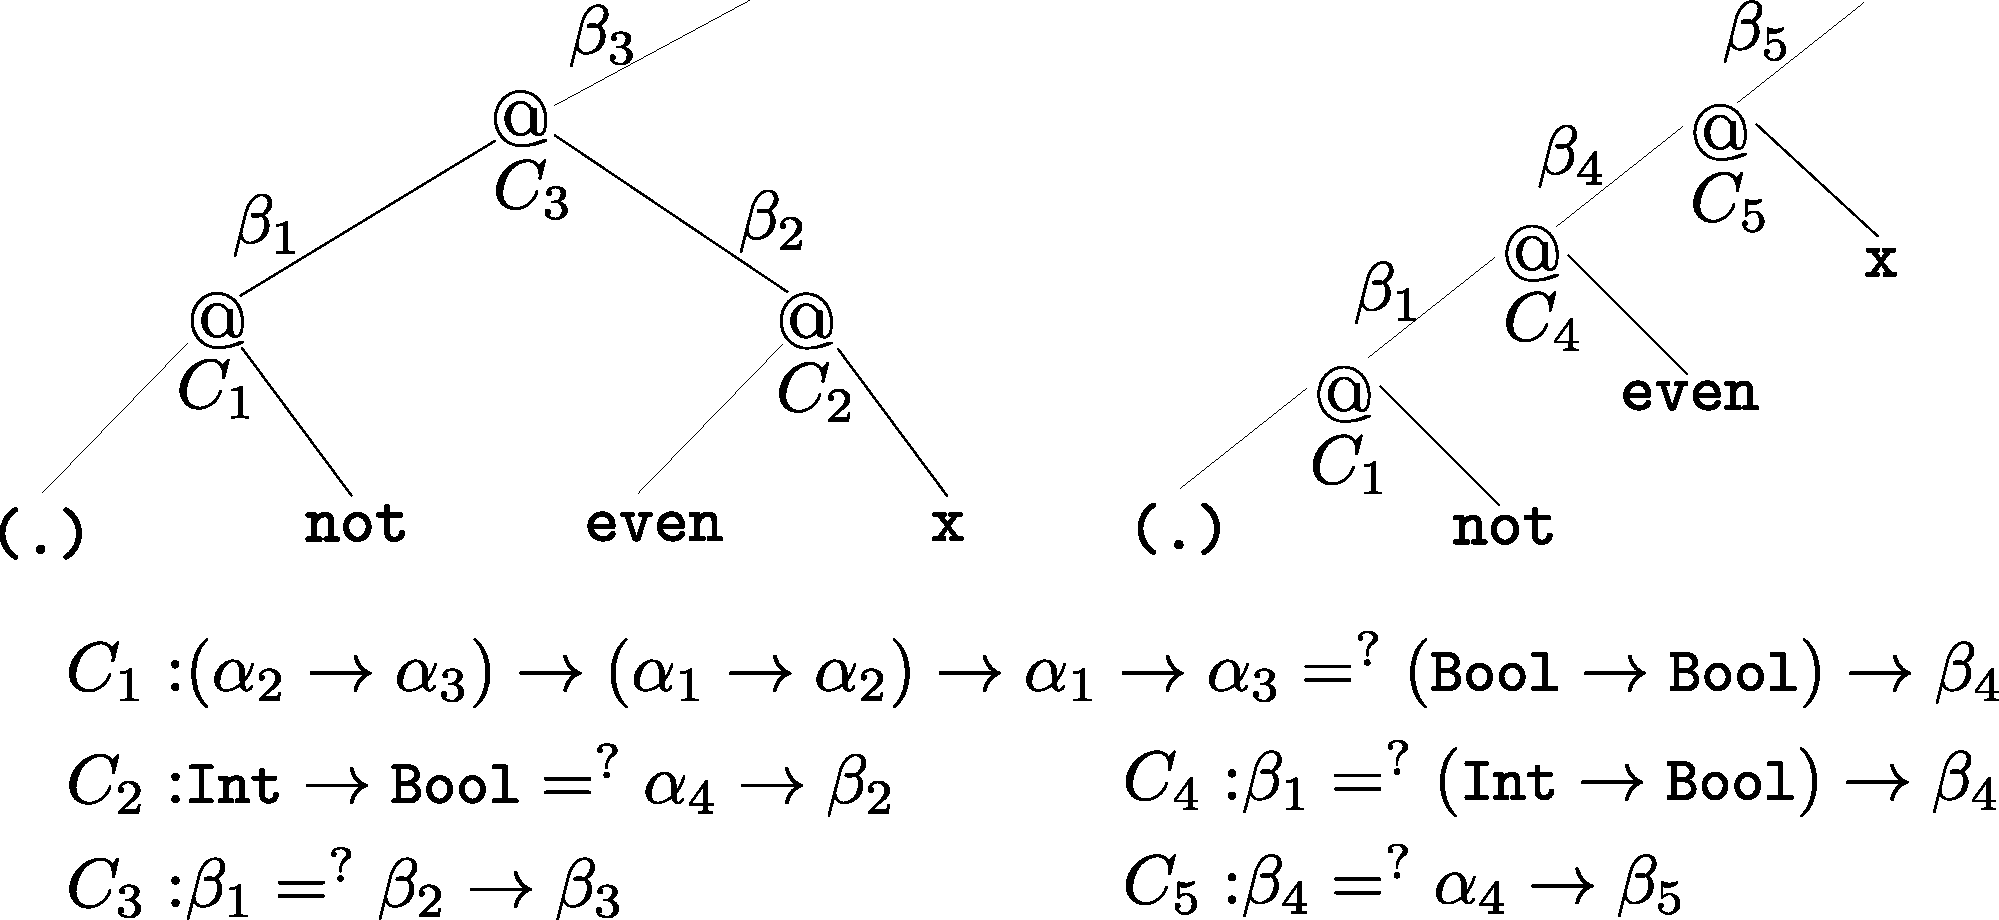
\includegraphics[width=0.85\columnwidth]{images/nonstruc.pdf}
\caption{The ASTs and constraints for \prog{not . even x} (left)
and \prog{(not . even) x} (right).
\ensuremath{@}s denote function applications.
The parameter \prog{x} has the type $\tvf$.
Annotations on edges denote types for the corresponding
subexpressions. For example, $\tvvf$ is the type for the
subexpression \prog{ (.) not}.}
\label{fig:nonstruc}
\end{figure}

A precondition for
constraint-based methods to work well is that the
faulty constraint is included in the given set of
constraints. However, this precondition fails
for the type errors caused by missing pairs of parentheses
or brackets.
For example,
consider debugging the type error for \prog{odd}
introduced in Section~\ref{sec:background:leaves:search}.
The \cs\ for \prog{odd} includes three constraints,
as shown in the left of Figure~\ref{fig:nonstruc}, where it
also presents the program AST. The constraints and AST for the
expected correct definition of \prog{odd} are shown in
the right of Figure~\ref{fig:nonstruc}. From the figure,
we observe that no constraint in \cs\ could be identified
as the faulty constraint such that changing the corresponding
subexpression would bring \prog{odd} to the
well-typed version, and consequently constraint-based debugging
methods fail to locate the real error cause. In this example,
both \toolH\ and \toolS\ blame the subexpression \prog{even x}
as the error cause.

%
For other non-leaf type causes, such as extra pairs
of parentheses, the precondition also fails to hold,
which makes constraint-based approach not work well.
We give evidence of this
for Helium in Section~\ref{xxx}.
%
In addition, constraint-based methods don't work well when there are
multiple error causes. One reason is that most
error debuggers try to report type errors in as few locations
as possible. As a result, even if the real error cause contains
multiple leaves, the debugger may return an error cause with
fewer leaves. For example, while the real error cause for
\prog{vulOp1} includes both \prog{(<)} and \prog{"~"},
Helium~\cite{Heeren05:TQT} suggests that the error cause
is \prog{replicate}.

Overall, constraint-based methods don't work well when a type
error is non-structural or involves multiple leaves.

\section{When Type Annotations Are Correct}
\label{sec:background:annotations}

While type inference can recover most omitted
type annotations, it is considered as a good
practice to add type annotations to at least
top-level bindings\footnote{http://en.wikibooks.org/wiki/Haskell/Type\_basics\#Type\_signatures\_in\_code}
for many reasons. As a form of documentation, type annotations improve
program readability. Compilers often exploit type annotations
to make type inference more efficient.

Type annotations also help to increase error
locating precision. For example,
the function \prog{vulOp} is
actually well typed if we remove its type annotation,
and it is the type annotation that helps error debuggers to detect
the type error in it. For this reason,
all GHC, Helium~\cite{Heeren03:HLH,Heeren05:TQT},
and \toolMin~\cite{Pavlinovic14:FMT,Pavlinovic15:PST}
treat user-specified type annotations as hard
constraints, meaning that they should always be trusted.
Once there is some error in type annotations, the
generated error messages is misleading, and following the
message will lead to more type errors in the program.
Thus, error debuggers work well when type annotations
are correct.

\chapter{Study Subjects and Methodology}
\label{sec:subjects}

In this chapter, I first describe the study subjects used in this work in Section~\ref{sec:subjects:db}.
Section~\ref{sec:subject:ref} discusses how the correct programs for ill-typed programs are determined.
At last, the information recorded to represent the real error debugging is presented in Section~\ref{sec:subject:metric}.

\newcommand{\benchf}{Haskell-1}
\newcommand{\benchs}{Haskell-2}
\newcommand{\bencht}{Haskell-3}
\newcommand{\benchl}{Haskell-3}

\section{Analyzed Datasets}
\label{sec:subjects:db}

A main challenge in this study is choosing appropriate data sets
for investigation. Since our goal is to study how type errors
were fixed, we need the data set to contain not only well-typed
programs but also intermediate ill-typed programs. This
requirement rules out most program data sets that teachers may
have collected while teaching functional programming, including those
offered through Massive Open Online Courses. In this work, we
use three Haskell data sets for our study. Figure~\ref{fig:datasets}
presents an overview of them.
%
For each data set, we give its name, the year it was collected,
%the programming language of the data set, 
the number of
programs in the data set, 
%
the number of program sequences in the data set 
(a sequence is the list of all programs from the same
student working on a specific assignment or exercise),
%
the number of ill-typed programs that
we investigated in the data set, the size range of programs
measured in LOC (Lines Of Code), the number of students
who took the corresponding course, and
the compiler that students used to compile programs.
%we used to compile each data set
%in the last column.

\begin{figure}[t]
\centering
\begin{tabular}{c | c c c c c c c}
Name &  Year     & No.\ progs & No.\ seqs & No.\ ill-typed   & Size  & No.\ students & Compiler\\
\hline
\benchf     & 2002  & 29,000 & 759 & 1,000 $\clubsuit$   & 2--190  & 119 & Helium \\
\benchs     & 2003  & 23,000 & 799 & 1,604       & 5--180 & 143 & Helium \\
\benchl & 2017   & 6,274 & 486   & 153 & 5--90 & 33  & GHC \\
\end{tabular}
\begin{center}
$\clubsuit$: The benchmark contains 2,000 ill-typed programs, and
we randomly analyzed 1,000 of them.
\end{center}
\caption{An overview of the data sets used for the study.}
\label{fig:datasets}
\end{figure}

The first two data sets were collected at Utrecht University,
and they included programs written
by first-year students learning the functional programming
language Haskell~\cite{jones2003haskell}, in years 2002 and 2003,
respectively. A copy of each program that
was compiled with Helium~\cite{Heeren03:HLH} and its
corresponding timestamp were recorded. These programs were written by
student to attempt to solve programming exercises or assignments, including
insertion sort,
string processing (such as calculating the maximum width of
strings in each column or padding each string in the table to
a certain length), boolean logic representations and operations, etc.
We defer detailed discussions about these program
sets to~\cite{Keeken06:AHP,Hage09:Neon}.

The data set \benchl\ was collected from an ongoing course. So far,
students in the course have worked on simple problems only, such as
representing binary values and converting them to decimal values,
computing Fibonacci sequences, determining whether lists are palindrome,
etc.

The ratio that the number of ill-typed programs
over the number of all programs
varies a lot across different data sets. In particular,
the ratio of ill-typed programs
%for \bencht\ is very high and that 
for \benchl\ is very low. 
This is because in this data set there is an
excessive number of well-typed programs that are similar,
which is potentially caused by 
the way how student
solutions are graded. The course uses an online
interface, where students submitted their solutions and received
feedback about whether their programs meet the assignment requirements immediately.
Usually students needs to finish an assignment by multiple steps,
and they can work on later steps only after passing the earlier steps.
Therefore, at each step students may keep on updating well-typed programs
until the running results of their programs are correct, yielding numerous
similar and well-typed programs.

For each data set, we used the compiler that was used in the class (last column in Figure~\ref{fig:datasets})
%
to compile each program,
collected the error messages for programs that have type
errors 
%but no unbound variables (since we can not decide what
%they were referring to), 
and analyzed the log file.
We did not consider programs that have unbound variables
because ignoring them does not affect our analysis results. 
We consider two cases when programs have unbound variables. 
In the fist case, 
%
the program do not contain any type error besides 
unbound variables. Such programs are irrelevant to 
our analysis. In the second case, the program does
contain type errors besides unbound variables. 
%
However, probably because Helium always reports 
unbound variable problems before reporting
type errors, students
always handled unbound variables first in such 
programs. Once the issue about unbound variables
was resolved, all type errors were exposed 
in the later versions of the student program, which we analyze.
Therefore, no information about type errors is missing
in our analysis. 

The program sets enable us to conduct our analyses 
at different scales.
To study how type errors were fixed,
we collected sufficient information 
by comparing each ill-typed program with its
corresponding student-intended well-typed program.
%which we call the \emph{reference program}. 
We discuss the
process of finding reference programs in detail in
Section~\ref{sec:subject:ref}.
%
To study what students did for fixing type errors,
we compared each ill-typed program with its next version of the program.
Moreover, by considering all the ill-typed programs over a period of several weeks,
we are able to study how the error fixing process evolved as students became more
familiar with the programming language.

\section{Finding the Reference Program}
\label{sec:subject:ref}

It is essential in our analysis procedure to choose,
for each ill-typed program,
a \emph{reference} program, which is the correct version of
the ill-typed program written by the same student.
Since identifying the reference program requires us to
understand the intention of the student
as well as the type error occurred in the program, it is impossible
to automate the procedure.
%just show that here we can use 'as a result' :)
As a result, we manually chose reference programs
to conduct the analysis on type error debugging.

%We discuss the process of how to choose the reference program in this subsection. 

%
%When a program contains multiple type errors,
%different type errors may be fixed in different references.
%different references may be
%used for fixing different type errors.



For each exercise finished by a student, we can
construct a \emph{program sequence},
including the student programs \pg{s}\ for the exercise,
the compiling results of \pg{s}, and the compiling time stamps.
%For simplicity, we use \seqijk\ to denote the
%program sequence for the exercise \pe.
%
%In manual analyses, we recorded various kinds of information
%to understand how type errors were fixed and what students did,
%detailed below.
%
Given a program sequence, denoted by \sseqijk,
we assume \pgi\ is ill typed, 
and \pgj\ is the first well-typed program after \pgi, 
and \pgk\ is another well-typed program after \pgj.
We follow the rule containing three cases below to
identify the reference program for \pgi\ in
the program sequence.
Without losing generality, we first illustrate the rule
by assuming that there is only one type error in \pgi.
After that, we show how to apply the rule to
find reference programs when \pgi\ has multiple errors.

%To identify the reference program of \pgi\ in the program sequence,
%we can follow the three steps below
%there are in general three different cases,
%and we present more likely case first as follows.

\paragraph{Case 1: \pgj\ is the reference for \pgi}
This is the most simple and straightforward case, 
where there is no intermediate well-typed program between 
\pgi\ and \pgj, and the programs after \pgj\ are not about 
fixing the type error in \pgi.
Take the student program sequence below as an example.\footnote{The original function had the Dutch name \prog{uitVullen}. To improve
readability, we have translated all Dutch names to English, except
for those we do not know how to translate or translation leads to name conflicts.}
The program is to make the string
\prog{s} up to a length of \prog{i} by
padding \progsq{\,}s.
%append a list of \prog{' '} at the end of a string.
We added the group and time information,
as well as the program name to the excerpt of each program in italics.
%
\begin{program}
fillOut :: String -> Int -> String \hfill \it{group103/2004-01-10@14_49_38_273 \quad p\textsubscript{1}}
fillOut s i = replicate (i - (length s)) " "

fillOut :: String -> Int -> String \hfill \it{group103/2004-01-10@14_50_10_811 \quad p\textsubscript{2}}
fillOut s i = replicate (i - (length s)) ' '

fillOut :: String -> Int -> String \hfill \it{group103/2004-01-10@15_51_33_552 \quad p\textsubscript{16}}
fillOut s i = s ++ (replicate (i - (length s)) ' ')
\end{program}
%
Both $\it{p\textsubscript{2}}$ and $\it{p\textsubscript{16}}$ are well typed, 
and $\it{p\textsubscript{16}}$ is the submitted version of the student program.
Based on the program sequence, we say
$\it{p\textsubscript{2}}$ is the reference of $\it{p\textsubscript{1}}$
because $\it{p\textsubscript{2}}$ is well typed,
and the changes after $\it{p\textsubscript{2}}$ are irrelevant to
the type error in $\it{p\textsubscript{1}}$,
and the final program $\it{p\textsubscript{16}}$ contains $\it{p\textsubscript{2}}$.

\paragraph{Case 2: \pgk\ is the reference for \pgi}
In this case, there exists the intermediate well-typed program \pgj\ 
between \pgi\ and \pgk, 
%\pgk\ is well typed, 
and the programs after the well-typed \pgk\ is not about fixing the type error in \pgi.
%
%In the second case, \pgk\ is the reference of \pgi, and \pgj\ is
%the intermediate well-typed program between \pgi\ and \pgk.
For example, \pgj\ might eliminate the type error
in \pgi\ by removing part of its ill-typed expression, and later
\pgj\ is changed into \pgk\ to have the expected functionality.
The type error in \pgi\ is relevant to the edits in \pgk,
while it is irrelevant to the further changes after \pgk.
Note that it is possible that there are multiple
intermediate well-typed programs
between \pgi\ and \pgk\ in a real program sequence.

%To better illustrate the second case, we use the following
%sequence from the program database as an example.
Consider the following sequence from the program database,
where 
\prog{Table} is defined as \prog{[[String]]} (In the whole
paper, \prog{Table} is a type synonym for \prog{[[String]]})
and \prog{widthColumn} is defined in the same program
and has the type \prog{Table -> [[Int]]}.
%
The function \prog{widthColumn} uses a matrix to store the length of 
every string in a \prog{Table},
and the function \prog{largestWidth} tries to compute the maximum
length of the string in each column of a \prog{Table}.
%We added the group and time information as well as the program
%name to the excerpt of each program in italics,
%and 
We omitted all the ill-typed programs between \pga\ and \pgc.
%
%and we use \prog{grootsteBreedte} as a short name for \prog{grootsteBreedte} in the original program.
%
\begin{program}
largestWidth :: Table -> [[Int]]  \hfill \it{group7/2005-01-10@12_36_57_499 \quad p\textsubscript{1}}
largestWidth t@(x:xs) = map maximum (transpose (widthColumn t))

largestWidth :: Table -> [[Int]] \hfill \it{group7/2005-01-10@12_37_33_561 \quad p\textsubscript{3}}
largestWidth t@(x:xs) = transpose (widthColumn t)

largestWidth :: Table -> [Int] \hfill \it{group7/2005-01-10@12_39_22_178 \quad p\textsubscript{6}}
largestWidth t  = map maximum (transpose (widthColumn t))
\end{program}
%
%\begin{program}
%\textit{group7/2005-01-10@12_36_57_499 \hfill p\textsubscript{1}}
%largestWidth :: Table -> [[Int]]
%largestWidth t@(x:xs) = map maximum (transpose (widthColumn t))
%
%\textit{group7/2005-01-10@12_37_33_561 \hfill p\textsubscript{3}}
%largestWidth :: Table -> [[Int]]
%largestWidth t@(x:xs) = transpose (widthColumn t)
%
%\textit{group7/2005-01-10@12_39_22_178 \hfill p\textsubscript{6}}
%largestWidth :: Table -> [Int]
%largestWidth t  = map maximum (transpose (widthColumn t))
%\end{program}
%\noindent
By removing the functions \prog{map} and \prog{maximum},
\pgb\ removes the type error in \pga. However,
\pgc\ is the correct reference program of \pga.
This is because no later changes after \pgc\ is relevant
to the type error in \pga, and
\pgc\ matches the student's intention according to
his/her final submitted program.

\paragraph{Case 3: no reference for \pgi}
%
We fail to find the reference program 
if the well-typed programs like \pgj\ or \pgk\
are not about fixing the type error in \pgi,
or if there is no well-typed program in the sequence.
There are two reasons that the reference does not exist in a program sequence.
First, the student gave up
fixing the type error and rewrote the whole code.
Second, the student switched to other compilers in later
versions~\cite{Keeken06:AHP} since using Helium was not mandatory.
We ignored such program sequences with no references since we are
not able to know students' intentions for them.
In our analysis, there are about 6\% of ill-typed programs
in the database we can not find their reference programs.

%strat to describe how the rule works for multiple errors with an example
%Considering an ill-typed program could contain more than one type error in practice,
%the way of finding program reference should be type-error based.
%
We now turn to the situation that a program may contain multiple
type errors. 
We use the following edit sequence of the program
\prog{printTable} to illustrate 
how the rule described above works to find reference programs
in this situation.
%when there are multiple type errors in a program.
%
%\begin{program}
%printTable :: Table -> String
%printTable (x:xs)   = printTableHeader x:xs ++ printTableContent tail (x:xs)
%\end{program}
%
\begin{program}
printTable :: Table -> String \hfill \it{group7/2004-02-02@11_28_36_363 \quad p\textsubscript{1}}
printTable (x:xs) = printTableHeader x:xs ++ printTableContent tail (x:xs)

printTable :: Table -> String \hfill \it{group7/2004-02-02@11_29_37_477 \quad p\textsubscript{2}}
printTable (x:xs) = printTableHeader x:xs ++ printTableContent (tail (x:xs))

printTable :: Table -> String \hfill \it{group7/2004-02-02@11_33_41_536 \quad p\textsubscript{7}}
printTable (x:xs) = printTableHeader x:xs

printTable :: Table -> String \hfill \it{group7/2004-02-02@11_40_16_149 \quad p\textsubscript{12}}
printTable (x:xs) = printTableHeader x

printTable :: Table -> String \hfill \it{group7/2004-02-02@11_43_52_864 \quad p\textsubscript{14}}
printTable (x:xs) = printTableHeader x ++ printTableContent (tail (x:xs))
\end{program}
%
%\begin{program}
%printTable :: Table -> String \hfill \it{group7/2004-02-02@11_28_36_363 \quad p\textsubscript{1}}
%printTable (x:xs) = printTableHeader x:xs ++ printTableContent tail (x:xs)
%
%printTable (x:xs) = printTableHeader x:xs ++ printTableContent (tail (x:xs)) \hfill \it{p\textsubscript{2}}
%
%printTable (x:xs) = printTableHeader x:xs \hfill \it{p\textsubscript{7}}
%
%printTable (x:xs) = printTableHeader x \hfill \it{p\textsubscript{12}}
%
%printTable (x:xs) = printTableHeader x ++ printTableContent (tail (x:xs)) \hfill \it{p\textsubscript{14}}
%\end{program}
%
In the program, \prog{printTableHeader} has the type \prog{Row -> String}, where \prog{Row} is defined as \prog{[String]}.
It intersperses all the strings in a row with
\progsq{+}s and concatenates them.  
%
The function \prog{printTableContent} has the type \prog{Table -> String},
and it intersperses all strings in a \prog{Table} with \progsq{|}
and concatenates them.
%
The function \prog{printTable} tries to append the results of \prog{printTableHeader} and \prog{printTableContent} together.
%
%

There are two type errors in the first program
$p\textsubscript{1}$, as can be seen by comparing it
with the final 
well typed program $p\textsubscript{14}$.
%
%We list the program sequence of \prog{printTable} as follows,
%and we show how to find the corresponding reference of each error.
%In the sequence, $p\textsubscript{12}$ is the intermediate well-typed program,
%and $p\textsubscript{14}$ is the final well-typed program.
%For simplicity, we omitted some unimportant steps in the sequence.
%
%
The second type error in the original program is removed in $p\textsubscript{2}$,
and the programs after $p\textsubscript{2}$ do not contain any changes 
related to \prog{printTableContent (tail (x:xs))}.
Therefore, $p\textsubscript{2}$ is the reference of the second error,
although the program itself is not well typed.
%
%
After the second type error is removed in 
$p\textsubscript{1}$, we can apply \textit{Case 1} above
to $p\textsubscript{1}$ to determine $p\textsubscript{12}$
as the reference 
for the first type
error in \prog{printTable}.
% is the last program $p\textsubscript{12}$. 
%The first type error is removed in 
%According to the rule, the reference of the first type error in 
%$p\textsubscript{1}$
%%the original program
%is $p\textsubscript{12}$.
%%
%Note that $p\textsubscript{12}$ is well-typed, 
%and it keeps the same in the student's submitted program $p\textsubscript{14}$.

Different errors in the same program may have different references.
Consequently, we study how each type error was fixed by investigating
the changes made, with respect to the error, between the original program
and the reference. We show more details about how the changes are measured
for each type error in the next subsection.

\section{Analysis Metrics}
\label{sec:subject:metric}

We constructed two records,
namely \emph{final fix} and \emph{fixing process},
for the analysis of how type errors were fixed and what students did, respectively.
Assume \pgi\ is the ill-typed program in \seqij, and \pgj\
is the reference of \pgi.
For the final fix record, we compare each \pgk\ with \pgj, where $k \in [i,j)$, 
and record the related information.
For the fixing process record, we compare each \pgk\ with $\pg_{k+1}$,
where $k \in [i,j)$, and record the related information.
In this subsection, we propose five metrics that
are used to represent the information in both records.

Before presenting the metrics,
it is important to note that a single metric may have
different meanings in different records.
Take the number of leaves changed in ASTs as an example.
In the final fix record, this metric reflects how
a program should
be changed to remove type errors.
%
In contrast, in the fixing
process record, it indicates what students did in
response to type errors.
Thus, the final fix record shows how type error debugging
looks like in practice while the fixing process record
reveals students' preferences and behaviors for fixing
type errors.


Next, we explain each metric used and how we measure it.
We use the following example \prog{maxLengte} to illustrate our calculations.
From this program on, we present the reference program in italics below the ill-typed program.
%
\begin{program}
maxLength :: [String] -> Int
maxLength x = maximum (map (length x))
\it{maxLength x = maximum (map length x)}
\end{program}
%
The error message generated by Helium is:
%
\begin{program}
(41,24): Type error in application
 expression       : map (length x)
 term             : map
   type           : (a -> b) -> [a] -> [b]
   does not match : Int      -> [Int]     
 because          : not enough arguments are given
\end{program}


Besides the reference program, number of fixing steps, 
and the creation date,
the measurements of the following metrics are recorded for each error.
Note that we focus on the place where
student changed to fix the type error.
%the changes made by students are directly
%related to the type error.
For example, in the program \prog{printTable}, although the student changed
the function \prog{printTableHeader} (called
by the function \prog{printTable}) 
during the debugging process,
we do not consider the 
leaf changes in it.


\begin{itemize}[noitemsep]

\item \textbf{Non-leaf/Leaf change}.
This metric represents whether the error cause is non-leaf or in leaves.
If it is non-leaf, we record the numbers of pairs of parentheses and
brackets that are added and
removed, respectively. 
Otherwise,
we record the number of leaves that are changed in program ASTs.
In the \prog{maxLength} example, for the
final fix record,
only one pair of parentheses was
removed,
and consequently it is Non-leaf change.


\item  \textbf{Correctness of type annotations}.
This metric reflects the reliability of type annotations in student programs.
We measure it by checking if the type annotation in the current program
is the same as the one in the reference.
In the \prog{maxLength} example, the type annotation is correct.
%This allows us to study the reliability of type annotations in type error debugging.

%\item The number of type errors in each ill-typed program.
%By recording how the number of type errors changes during the fixing process,
%we are able to discover the behaviours of students for dealing with multiple type errors.

\item \textbf{Size difference}.
This metric is the sum of the size of the expression
that is changed from in the original program
and
that of the expression that is 
changed to in the reference program. 
We use the notation $n$--$m$ to denote that
$n$ nodes and $m$ leaves in the AST are changed.
This metric measures how close the two
expressions are: the larger is this value, the more efforts are needed to
make the change.
In the \prog{maxLength} example, 
the expression changed from is
\prog{map (length x)} and that changed to is \prog{map length x}.
Their sizes are 3--2 and 3--2, respectively.
Therefore, the size difference is 6--4.
%Similarly, the size difference for the second error is 14--8.
% based on the modified program excerpt \prog{tail (x:xs)}.
%By observing this information over multiple steps in the program sequence,
%we can decide if ill-typed programs are increasingly close to their
%references or there is a diverging phase in fixing process.

\item \textbf{Helium information}.
For this metric, we consider:
\begin{enumerate*}[label=(\alph*)]
\item does Helium locate the real error cause correctly,
\item whether following Helium's change suggestion will bring
the current program to the reference program,
\item the distance between the real error cause and the one reported
by Helium in terms of the number of identifiers, and
\item the category of the change suggestion.
\end{enumerate*}
%
We extract these items by investigating the current program,
the reference program, and the Helium error message for the corresponding error.
For example, the results for items (a), (b), and (c)
in \prog{maxLength} are ``no'', ``no'', and 1, respectively. 
We discuss item (d) in detail in Section~\ref{sec:effectiveness}.
%
The purpose of this metric is not to evaluate the quality
of error messages of Helium, but rather to study how
the precision of error locating and different message categories 
affect the error debugging in practice.
%\item Number of intermediate correct programs.
%We count the number of correct programs
%between the ill-typed program and the reference program.
%This, together with some other information about
%the corresponding correct programs like the changes of expression sizes,
%allows us to investigate how students work toward the well-typed programs.

%\item Whether the expression is the same as before.

\item \textbf{Difficulty reason}.
Debugging difficult type errors usually takes
students more steps or more time.
We summarize the difficulties based on different aspects of language features,
namely \emph{type annotations},
\emph{library function usage}, \emph{function composition},
\emph{point-free function}, and \emph{pattern matching}. 
We discuss more details of the difficulty reasons in
Section~\ref{sec:difficulty}.
This metric
allows us to discover which language features are difficult to students
with respect to type error debugging.
For example, the student took 9 steps to fix the type error in \prog{maxLength},
and the difficulty is due to the wrong function composition of \prog{map} and \prog{length x}.

\end{itemize}


\noindent
For final fix, all these metrics are used in the work. For
fixing process, only the metric Non-leaf/Leaf change is used
in Section~\ref{sec:causes}.


\chapter{Debugging Behavior Analysis}
\label{sec:analysis}

This chapter presents the analysis results based on the three datasets introduced in Section~\ref{sec:subjects:db}.
A bird's-eye view of the findings about students' debugging process is first provided in Section~\ref{sec:overview}.
Then, I present the statistical results of error locations (Section~\ref{sec:causes}), type annotation reliability (Section~\ref{sec:annotation}),
error message effectiveness (Section~\ref{sec:effectiveness}), and difficult language features (Section~\ref{sec:difficulty}) in the respective section. 
At last, I discuss the threats to validity in Section~\ref{sec:threat}.

\section{Overview of Error Debugging in Practice}
\label{sec:overview}

\begin{figure}
\centering
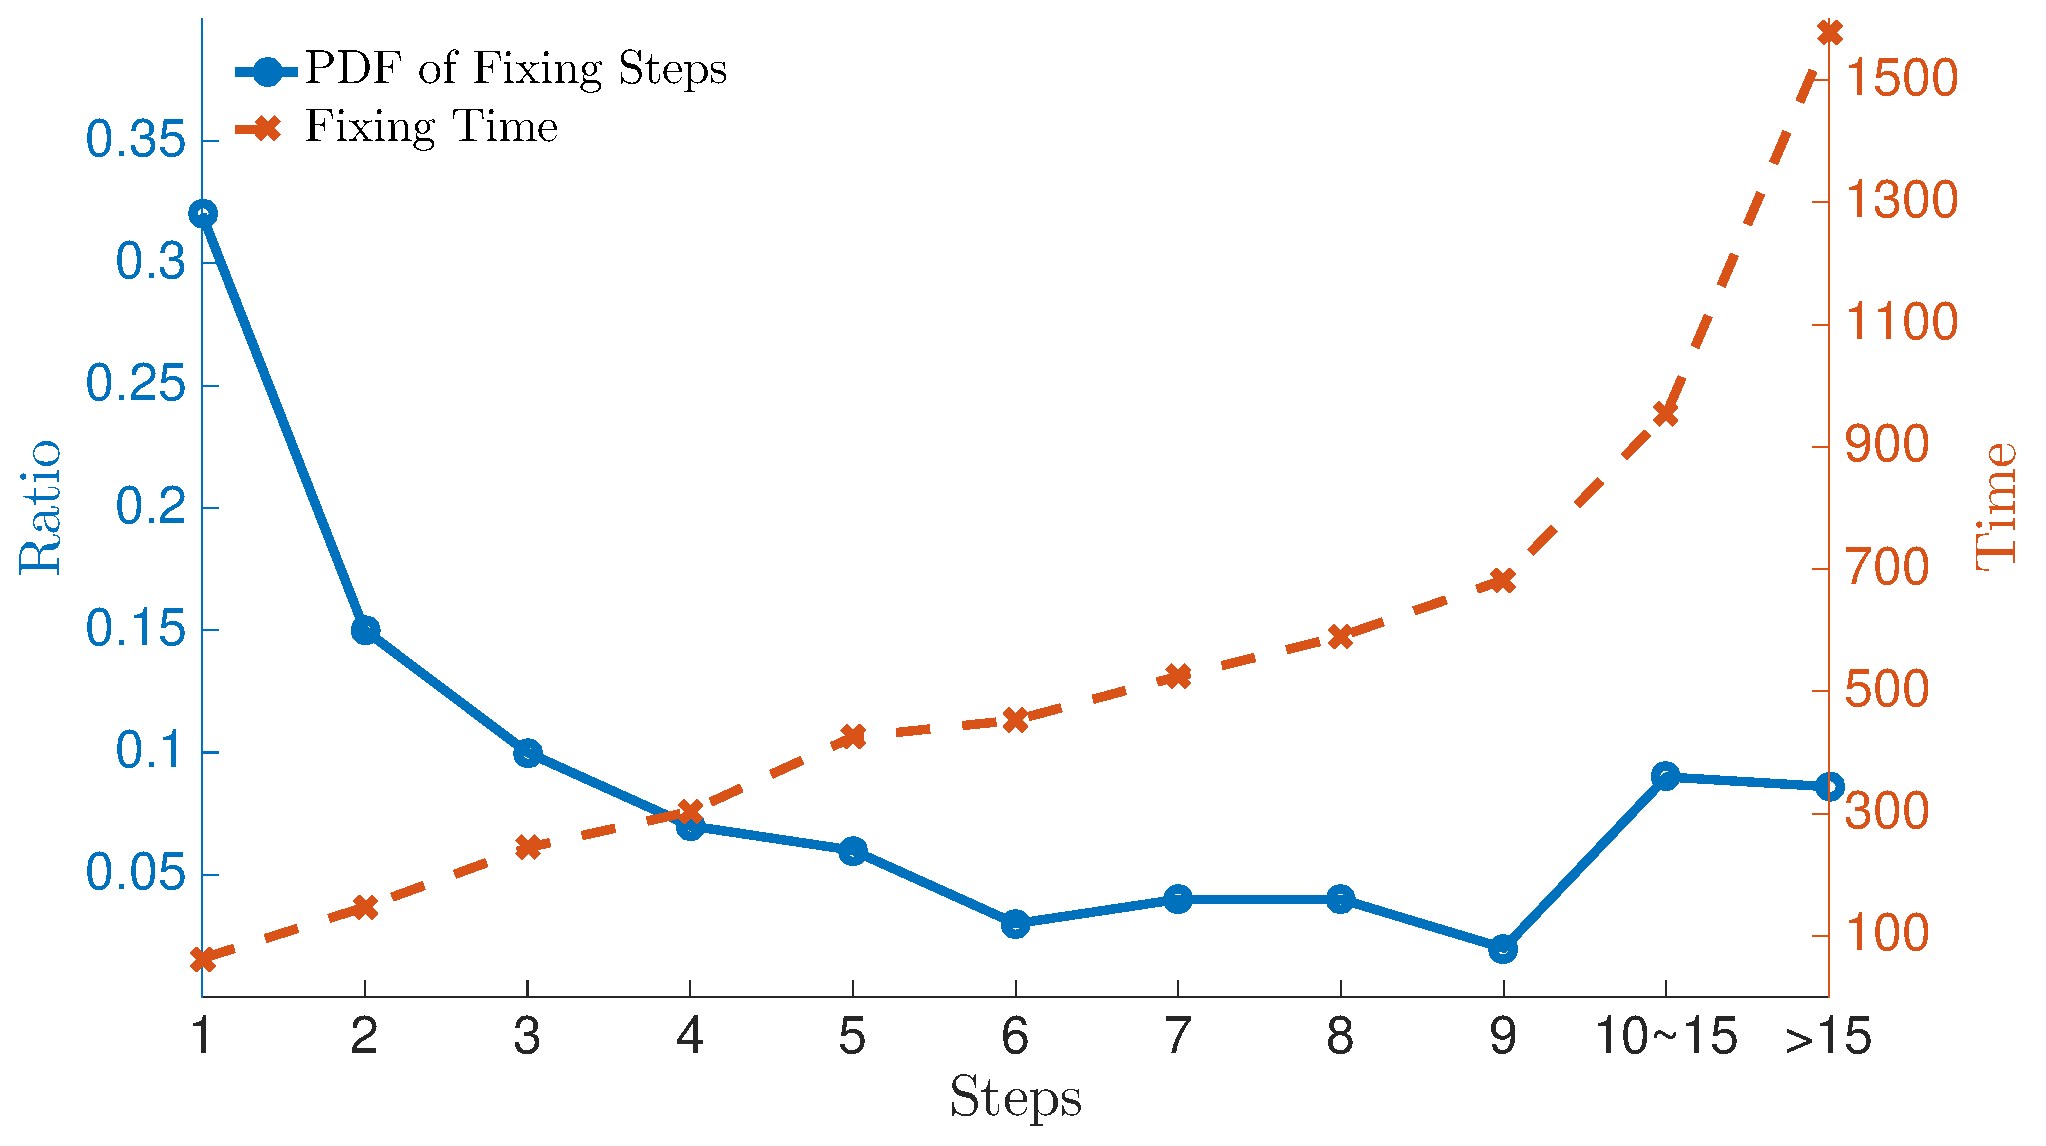
\includegraphics[width=.85\columnwidth]{images/step_time.eps}
\caption{Fixing steps and times in program data sets}
\label{fig:fst}
\label{fig:overview:overview}
\end{figure}

In this section, we present an overview about the number
of steps and time duration students spent on fixing
type errors by considering the three data sets
together. We also show how they evolve over an eight-week
period. 
%
Figure~\ref{fig:fst} shows the distribution of 
fixing steps, where any point $(x,y)$ on the 
solid curve denotes that the ratio of type errors
fixed with $x$ steps over all the type errors is
$y$. 
%
%
For example, (1,32\%) indicates that 32\% of all type
errors are fixed within a single step. 
%There are 32\% of the errors fixed by one steps, 
%which is the most common case in debugging situations.
%
The ratio decreases as the number of fixing steps increases.
%
While many type errors are fixed within a couple of 
steps (probably due to some obvious mistakes that are easy
to fix), 
a large portion of type errors required
more steps to fix.
For example, about 30\% of the errors took more than 5 steps to fix,
and 18\% of the errors took more than 10 steps to fix.
In average, the number of fixing steps 
is 4.7 (\std \footnote{\std\ is the standard deviation}=6.2)
for \benchf,
5.8 (\std=8.0) for \benchs, 
and 4.3 (\std=5.1) for \benchl.
Here we have large standard deviations because 
the data sets contain large variations of error fixing
situations. For example, many type errors were fixed with
just 1 or 2 steps while others might take more than 15 steps.


Figure~\ref{fig:fst} also shows the relation 
between time duration and the number of fixing steps.
To increase the readability, we show only the average
time for each number of fixing steps in the figure. 
%
In general, the time increases as the number 
of fixing steps increases. 
For example, students spent 63 seconds on average
for errors that are fixed with a single step,
425 seconds for errors fixed with 5 steps,
and 842 seconds for those fixed with 10 steps. 
%
The correlation coefficient between 
fixing time and the number of fixing steps
is 0.81 with the \emph{p}-value $< 1e^{-13}$ (
the correlation coefficient is computed 
based on all fixing duration with respect to fixing steps).
As the correlation is strong,
we can either use the number of fixing steps
or fixing time to reflect the difficulty of error debugging  in our later discussions.


\begin{figure}
\centering
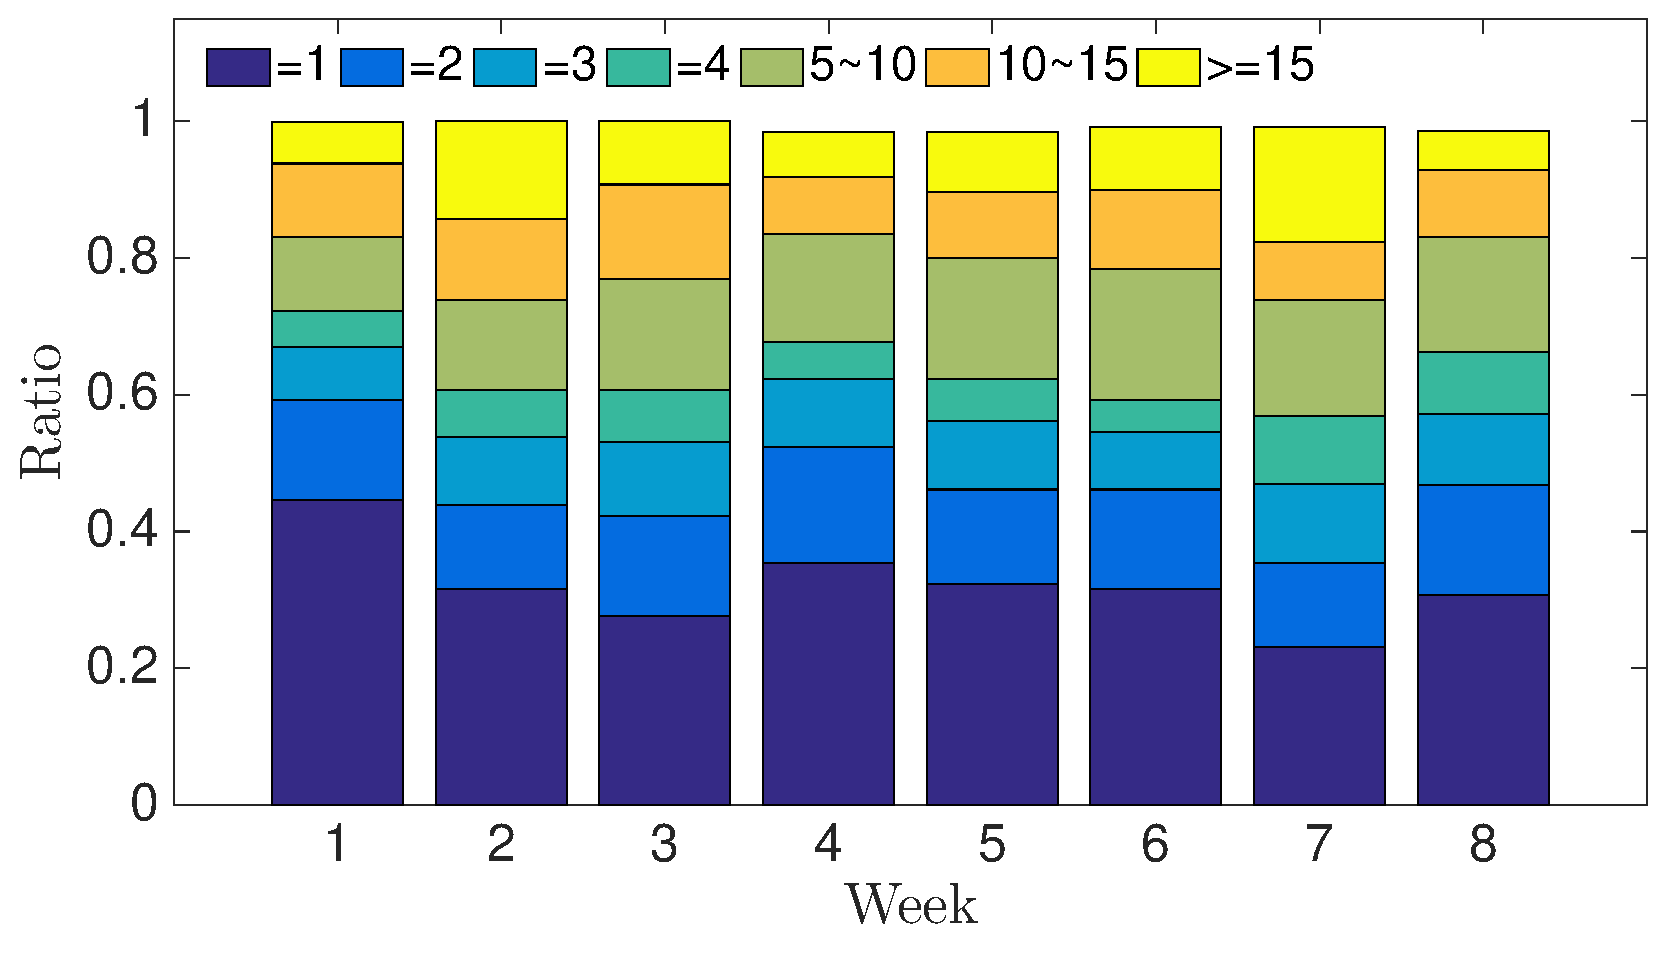
\includegraphics[width=0.85\columnwidth]{images/step_time_ratio_1.eps}
\caption{Distribution of fixing steps over the time}
\label{fig:sot}
\label{fig:overview:dos}
\end{figure}


Figure~\ref{fig:overview:overview} shows that the numbers
of fixing steps vary a lot. We are also interested in knowing
if this variability was preserved over time.
Specifically we want to know 
if students tended to have longer error
debugging sequences when they first started to learn the language
while have shorter 
sequences as they became more experienced 
with the language
and type error debugging.
%
%it does not tell whether
%time points (such as the first or last week) are relevant.
%
Figure~\ref{fig:sot} 
addresses this question
by showing 
the evolution of the numbers of fixing steps
over an eight-week period.
The figure considers \benchf\ and \benchs\ together.
For each week, we compute the ratio for each number
of fixing steps. 
%different fixing steps (e.g. step=1 or 5$\leq$step$<$10) in each week.
For example, the ratios of one-step fixes
range from 0.25 to 0.44 during week 1 to 8,
and the average ratio is 0.32 (\std=0.06). 
The value of \std\ is small, meaning that
one-step ratios do not change much over the time.
We have similar results about \std\ for other numbers of 
fixing steps. 
%
Therefore, the distribution of
different numbers of fixing steps is quite stable as time went by.


\cite{hage2006mining} shows
that the number of type errors students made in most
weeks are similar (except that
week one had fewer and week three had more
type errors). Together with the result in
Figure~\ref{fig:overview:dos}, we can conclude
that, type error debugging was consistently 
challenging over time for students, even after they
had been programming in Haskell, reading error messages,
and fixing type errors for several weeks. 

\section{Where Were Error Causes?}
\label{sec:causes}

In Section~\ref{sec:background:leaves}, we discussed that most error debuggers work well
when type errors are caused by single leaves.
In this section, we investigate how programs were fixed
by grouping all programs according to the number of leaves that
were changed. We write $n$-leaf to mean that $n$ leaves
were changed and write non-leaf to mean that
pairs of parentheses or brackets were added or removed. Our discussion assumes
that each program contains one type error only.
When a program contained multiple errors, we considered the type errors
individually.

\begin{figure}
    \centering
    \begin{subfigure}[t]{0.75\textwidth}
        \centering
        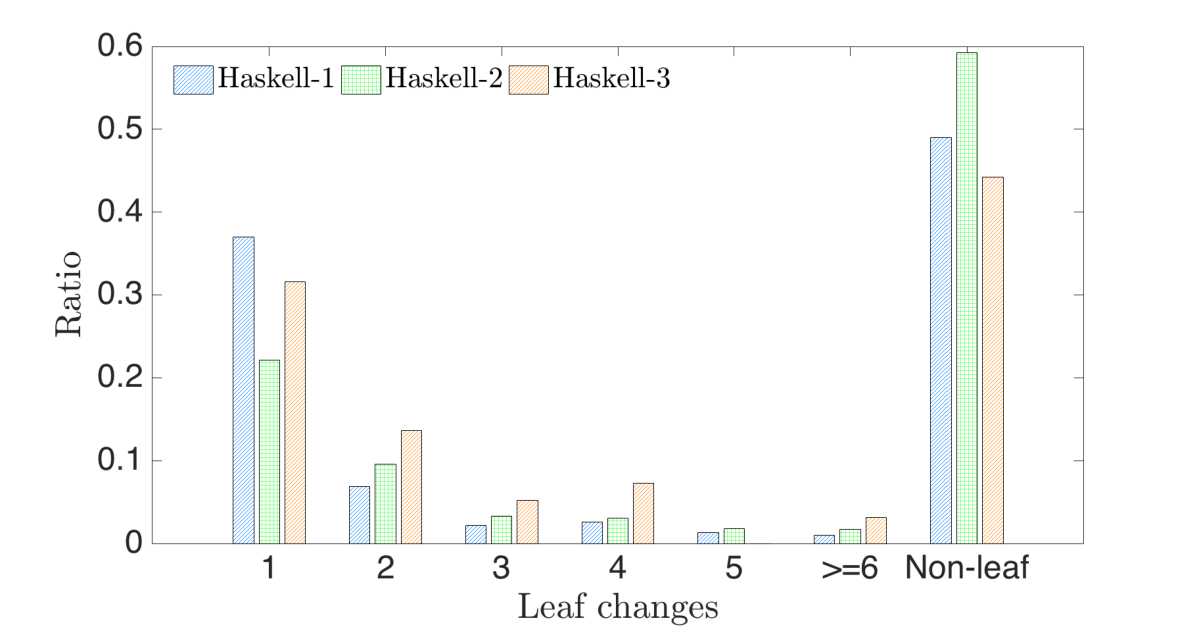
\includegraphics[width=0.97\columnwidth]{images/leaf-final.pdf}
        \caption{Distribution of leaf changes in final fix}
        \label{fig:leaf-chg-dist:final}
    \end{subfigure}
    
    \begin{subfigure}[t]{0.75\textwidth}
        \centering
        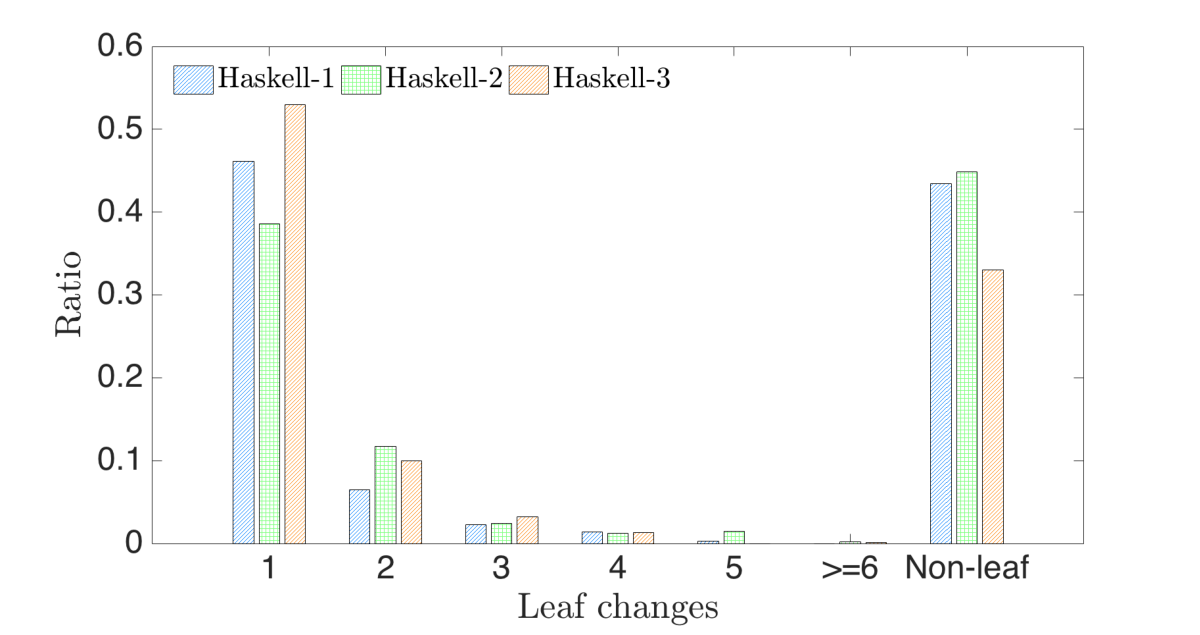
\includegraphics[width=0.97\columnwidth]{images/leaf-process.pdf}
        \caption{Distribution of leaf changes in fixing process}
        \label{fig:leaf-chg-dist:proc}
    \end{subfigure}%
    \caption{Distribution of leaf changes}
    \label{fig:leaf-chg-dist}
\end{figure}

Figure~\ref{fig:leaf-chg-dist} shows the distribution of
programs with respect to the number
of changed leaves in both the final
fix (Figure~\ref{fig:leaf-chg-dist:final})
and fixing process
(Figure~\ref{fig:leaf-chg-dist:proc}) records.
%
The ratio for $n$-leaf is calculated by dividing the number of
programs that belong to $n$-leaf over the number of all
ill-typed programs.
%
As we can see from Figure~\ref{fig:leaf-chg-dist:final},
non-leaf changes always account for the majority
of all kinds of leaf changes across different data sets. 
Specifically, the ratio of non-leaf change in \benchs\
reaches more than 50\%,
and the ratios are more than 45\% in the other two data sets.
In other words, more than
45\% of type errors were fixed
by adding or removing pairs of parentheses or brackets
in all data sets.
%
In contrast, for 1-leaf change, where existing debuggers work
well, its ratio ranges from only about 22\% in \benchs\ to about 37\%
in \benchf.

%
%
Figure~\ref{fig:leaf-chg-dist:proc} shows where students preferred
to make changes when fixing type errors. An interesting observation
is that, across all data sets, students made changes with respect to single leaves  
more often than non-leaf changes during fixing process. 
For example,
students made 1-leaf changes for about 39\% of all errors in \benchs,
while only about 21\% of changes were non-leaf.
Moreover,
the ratio of non-leaf changes is decreased from fixing
process to final fix in all data sets. For example, for \benchs,
the ratio is decreased from 60\% to 45\%.
%
These numbers imply that
either students were unaware of the high frequency of causing type
errors by wrong pairs of parentheses or brackets,
or they were misled by the error messages when type errors were non-leaf.
%
Consider, for example, the program \prog{maxLength} introduced in Section~\ref{sec:subject:metric}.
We can observe that actually the student got all the necessary identifiers (\prog{map},
\prog{length}, and \prog{x}) right but had an extra pair of
parentheses.
Unfortunately, the error message pointed to a wrong direction,
making the student take 9 steps to identify the real error cause.
This example shows that error debuggers fail to
convey information accurately
when type errors are not at leaves.

\begin{figure}
\centering
    \begin{subfigure}[t]{0.75\textwidth}
        \centering
        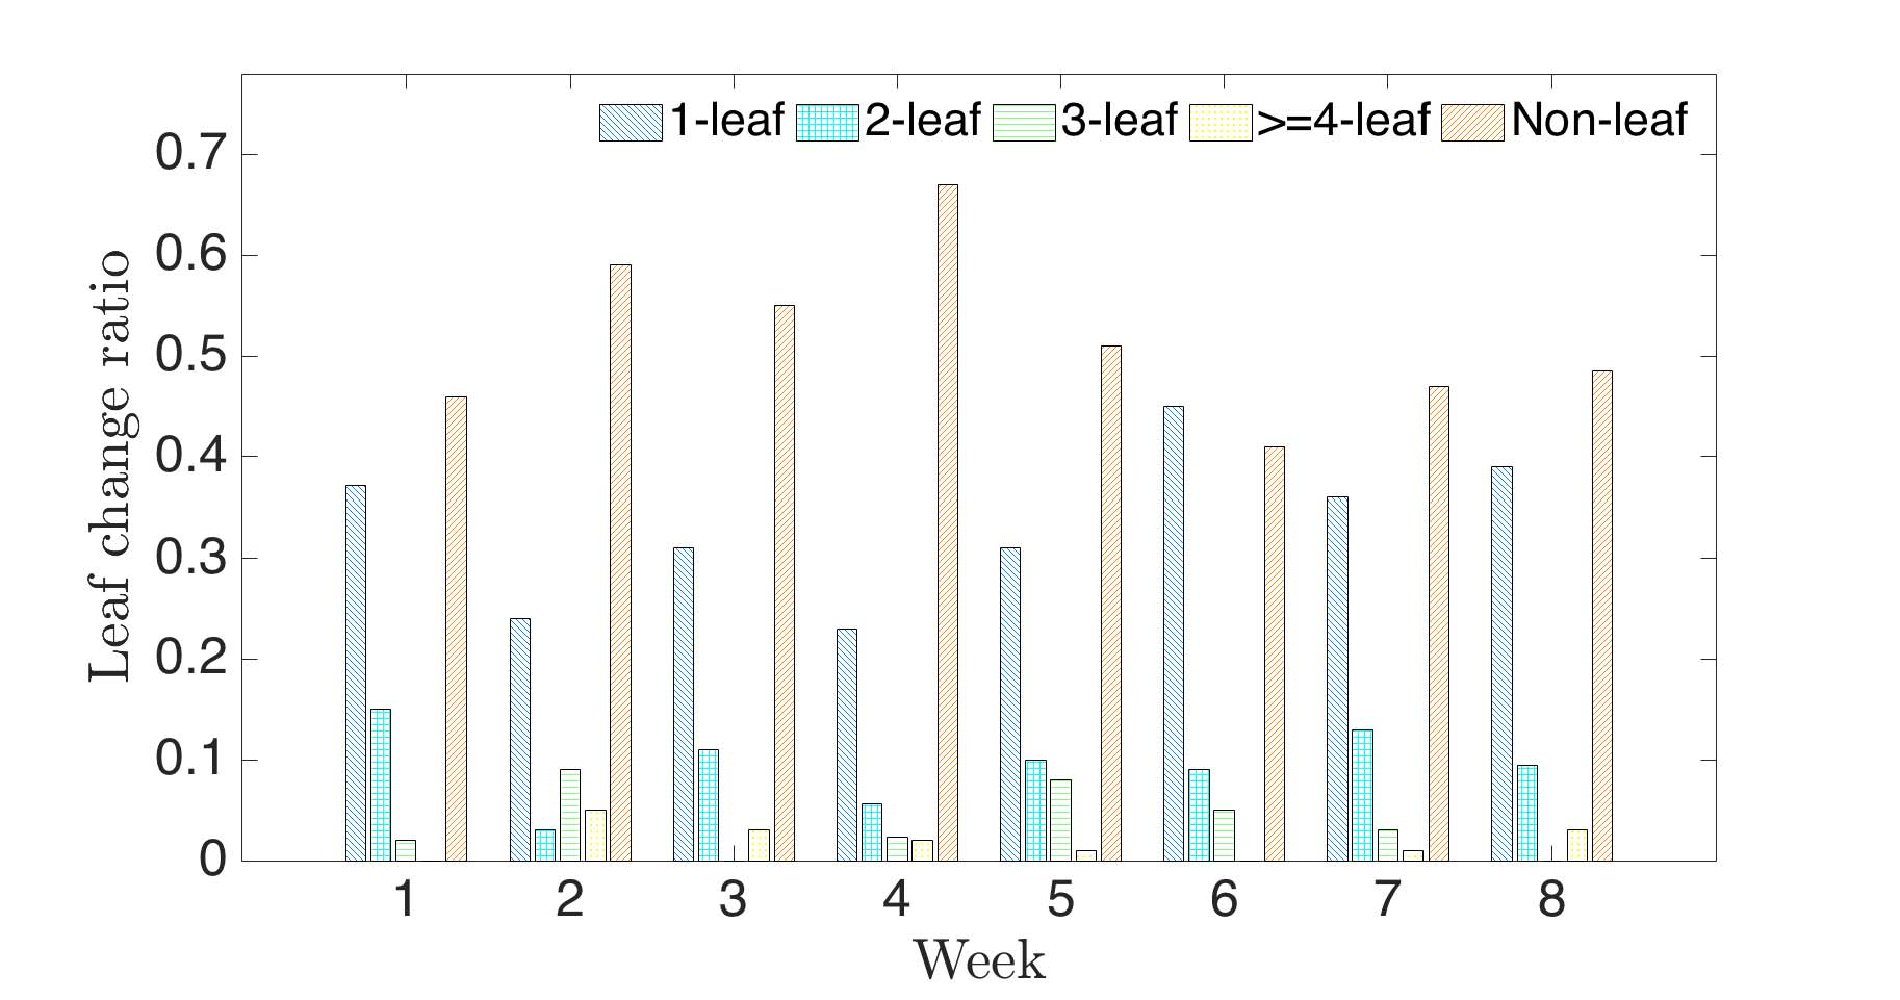
\includegraphics[width=0.97\columnwidth]{images/lt02.pdf}
        \caption{Evolution of leaf changes for \benchf}
        \label{fig:leaf-chg-evol:data1}
    \end{subfigure}%
    
    \begin{subfigure}[t]{0.75\textwidth}
        \centering
        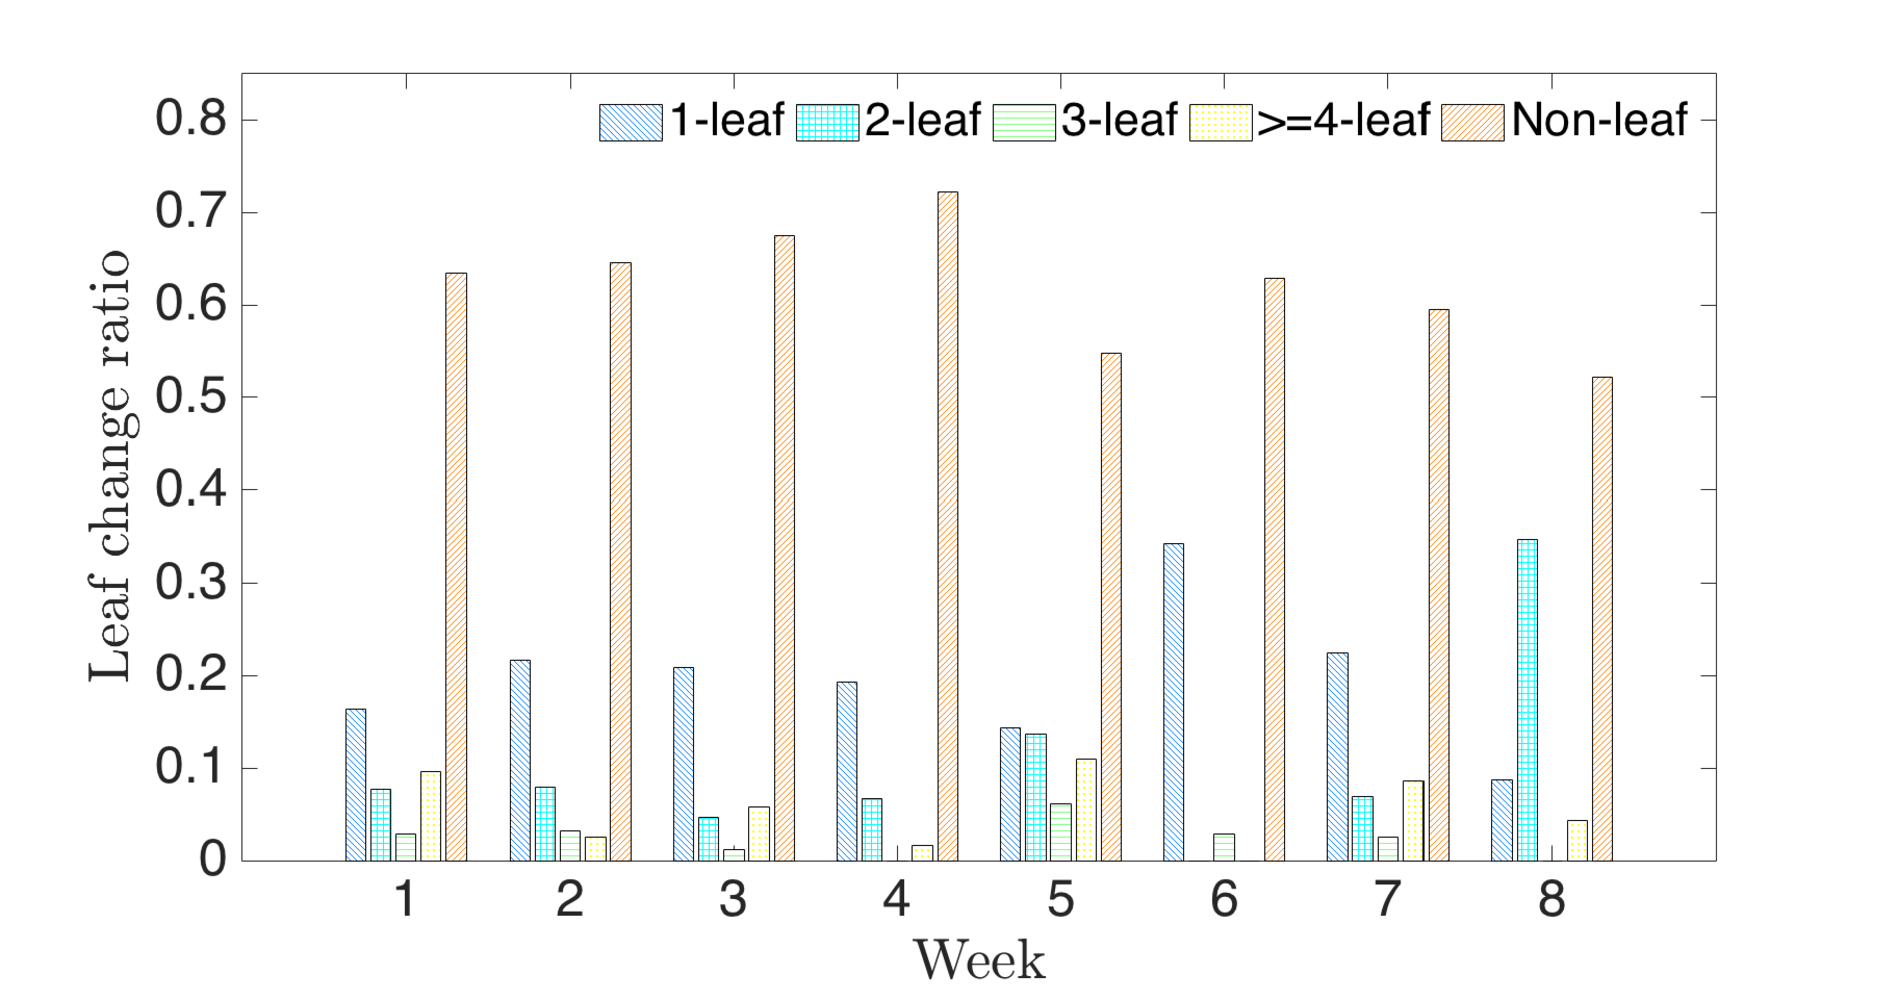
\includegraphics[width=0.97\columnwidth]{images/lt.pdf}
        \caption{Evolution of leaf changes for \benchs}
        \label{fig:leaf-chg-evol:data2}
    \end{subfigure}

    \caption{Evolution of leaf changes against weeks}
    \label{fig:leaf-chg-evol}
\end{figure}

Figure~\ref{fig:leaf-chg-evol} shows the evolution
of the ratios 
%of different kinds 
of leaf changes in the
final fix record. 
Note that week 1 denotes the
first week students submitted programs, not necessarily the
first week in the corresponding semester.
%In Figure~\ref{fig:leaf-chg-evol:data3}, we skipped the weeks
%that students had no submission in them. Also
We don't have such an evolution figure for \benchl\ because the
course is still ongoing and we had data for only 3 weeks.
%
%In particular,
%in all but only one week across all data sets, type errors were fixed
%more often by adding or removing parentheses than by changing
%single leaves. 
We observe that the ratio of non-leaf changes
ranges from 50\% to 70\%
while the ratios of 1-leaf change are always less than 40\% in \benchs.
For \benchf, we have a similar observation that the ratio of non-leaf changes is higher
than that of 1-leaf changes in most weeks. 
These figures again show that
most of the errors were not caused by single leaves in ASTs,
although the ratios vary from week to week.
Combined with our discussion in Section~\ref{sec:background:leaves},
the results in Figures~\ref{fig:leaf-chg-dist} and~\ref{fig:leaf-chg-evol}
indicate that most existing error debuggers may not work well in
real debugging situations.
%at least they are not able to locate type errors accurately in the student programs.


Figure~\ref{fig:lst} shows 
%how the number of fixing steps changes with
%different kinds of leaf changes.
the relation between the number of leaves changed and the number of steps to fix the type error.
%
Not surprisingly, the median value of the number of
fixing steps increases as more leaves are changed
in final fix.
The correlation values between fixing steps and leaf changes
in \benchf, \benchs, and \benchl\ are 0.423 (\emph{p}-value=$13e^{-15}$),
0.518 (\emph{p}-value=$1e^{-15}$), and 0.451(\emph{p}-value=$1e^{-15}$), respectively.
The results tell that students need more steps to fix type errors involving more leaves,
since the corresponding error messages become less 
%accurate and 
effective.
We also note that the numbers of fixing steps for non-leaf errors
are usually greater than those for $n$-leaf errors in 
all the three data sets.
For example, in \benchs, the median value of the number of 
fixing steps for 
non-leaf error is about 5, while those for 1-leaf and 2-leaf error
are about 1 and 4, respectively.
In addition, about 14\% of non-leaf errors take
students more than 15 fixing steps.
The result shows that type errors
that are not caused by leaves are
most difficult for students to fix.


\begin{figure}
\centering
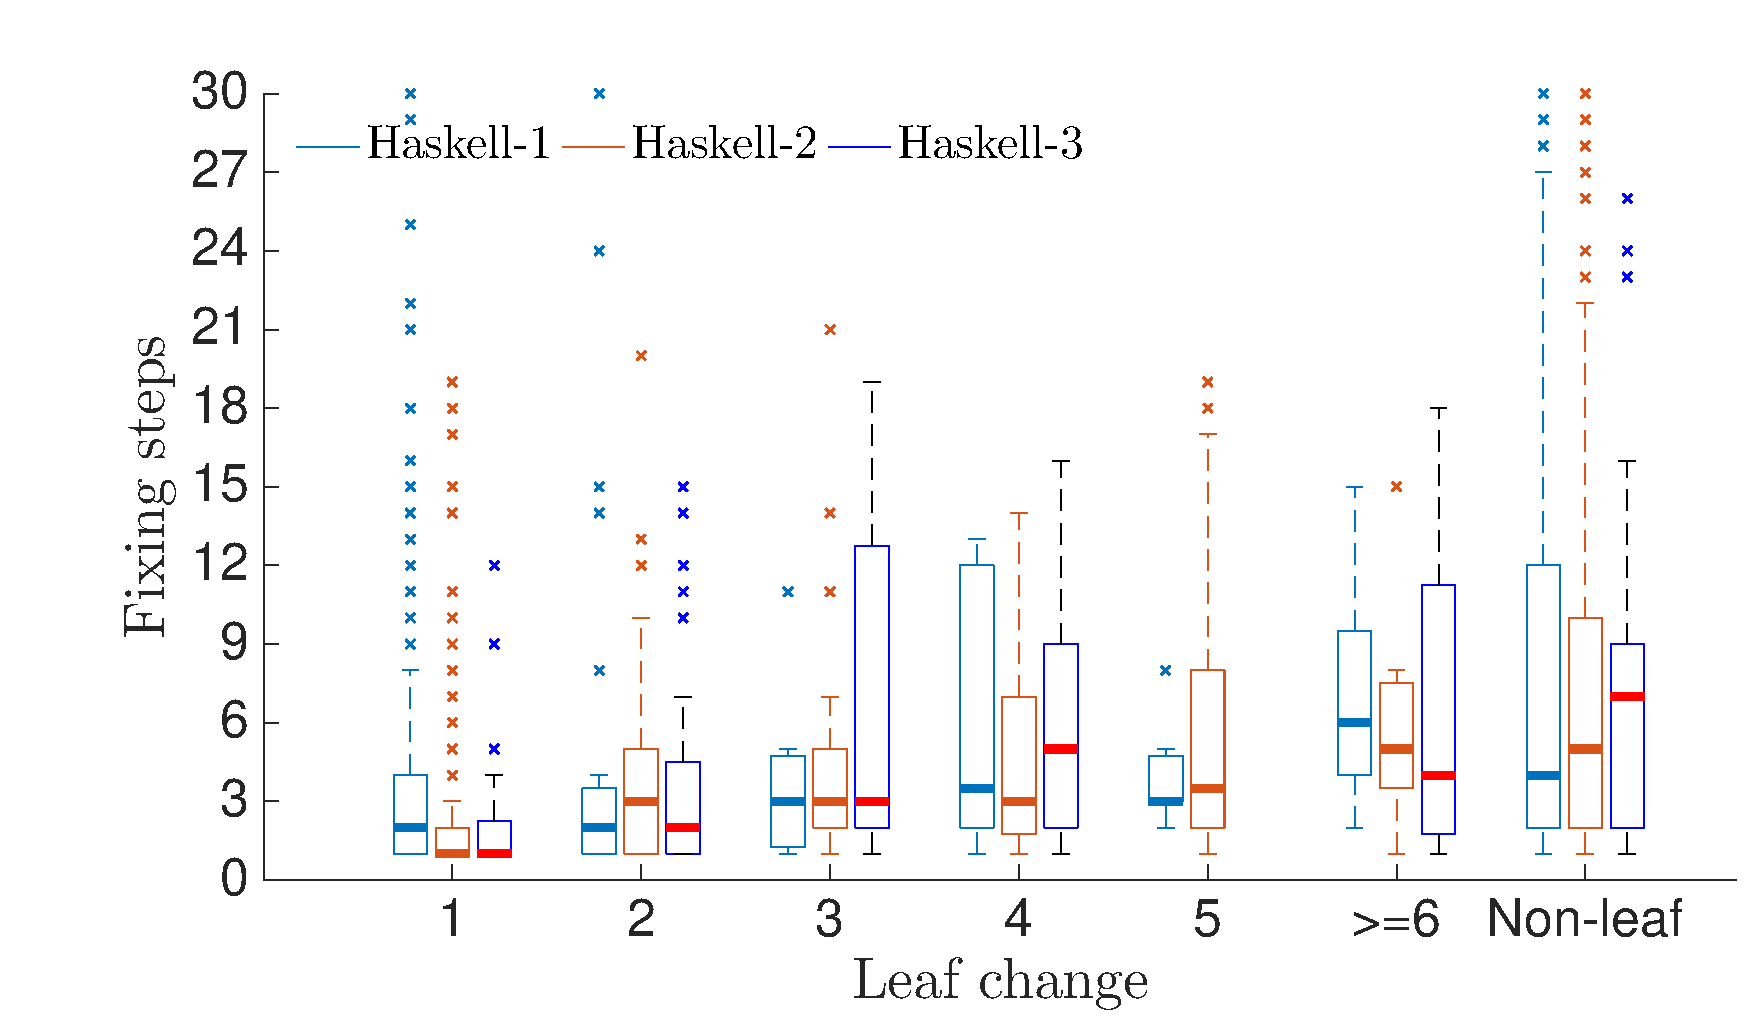
\includegraphics[width=.85\columnwidth]{images/leaf_step.eps}
\caption{The relation between leaf changes and the
number of steps to fix the type error}
\label{fig:lst}
\end{figure}

We conclude that in practice most error
debuggers won't work well since
type errors are
often not caused by single leaves.
Seminal could search for type errors that
are not caused by leaves
%the causes that are not at leaves for type errors,
but it does not achieve a high error locating
accuracy~\cite{Zhang14:tgd,CE14popl}.
Therefore, it would be useful to develop
an error debugger that fixes non-leaf errors
systematically.

\newcommand{\years}{\benchf}
\newcommand{\yeart}{\benchs}

\section{Were Type Annotations Reliable?}
\label{sec:annotation}

Since compilers and many error debuggers always trust type annotations,
it is important to study the reliability of type annotations.
%
%
In this section, we define the ratio of wrong type annotations
as the number of type errors containing 
%We first investigate the ratio that students made mistake on type annotations
%as the number of type errors containing 
wrong type annotations 
over the number of all type errors.
%
Based on the final fix record, the ratio of wrong type annotations
is 28\% 
for \benchf, 34.4\% for \benchs, and 
27\% for \benchl. 
%
The result means that, in general, error debuggers can not
precisely locate the real error causes for around 30\% of
type errors if they always trust type annotations. 

The ratio is surprisingly high,
and we investigated why this happens.
%
We found out two main reasons that cause wrong type annotations
to appear frequently.
The first one, called wrong definitions, is that
students wrote wrong type annotation at the beginning.
The other, called out-of-synchronization,
is that students forgot to update type annotations
after they changed the related function definitions.
For example, in \benchs, the ratios for wrong definitions and
out-of-synchronization are 31.3\% and 30.6\%,
respectively.


\begin{figure}[t]
\centering
\begin{tabular}{  c | c | c | c | c | c | c | c | c | c }
\toprule
  Week & 1 & 2 & 3 & 4 & 5 & 6 & 7 & 8 & Average of weeks\\
\midrule
  \benchf & 0.18 & 0.29 & 0.36 & 0.38 & 0.36 & 0.26 & 0.28 & 0.28 & 0.30 (\std=0.07) \\ 
  \benchs &  0.16 & 0.23 & 0.43 & 0.41 & 0.53 & 0.29 & 0.25 & 0.26 & 0.32 (\std=0.12)  \\ 
\bottomrule
\end{tabular}
\caption{Ratio of wrong type annotations}
\label{fig:at}
\end{figure}

We are also interested in knowing if
the ratio of wrong type annotations will be affected
as students were more exposed to
%became more familiar with 
functional programming and the language.
In Figure~\ref{fig:at}, we present the ratio of 
wrong type annotations of each week in
\benchf\ and \benchs. We do not present the
result for \bencht\ because it covers only
three weeks so far.
%
In the first week,
the ratios of wrong type annotations in both program data sets are low
since the programming assignments were simple
and the programs were small~\cite{Hage09:Neon}.
After week 1, students started to make more wrong type annotations
as the assignments became more difficult.
In particular, the highest ratio
in \benchf\ is 0.38 (in week 4) and that in
\benchs\ is 0.53 (in week 5).
%
In later weeks, as students 
were exposed more to Haskell programming,
the ratio of wrong type annotation decreased a little. 
Nevertheless, the average ratio over 8 weeks is about 30\% with relatively small \std\ in both data sets,
which implies that wrong type annotations 
seems to be a constant problem.


\begin{figure}
\centering
%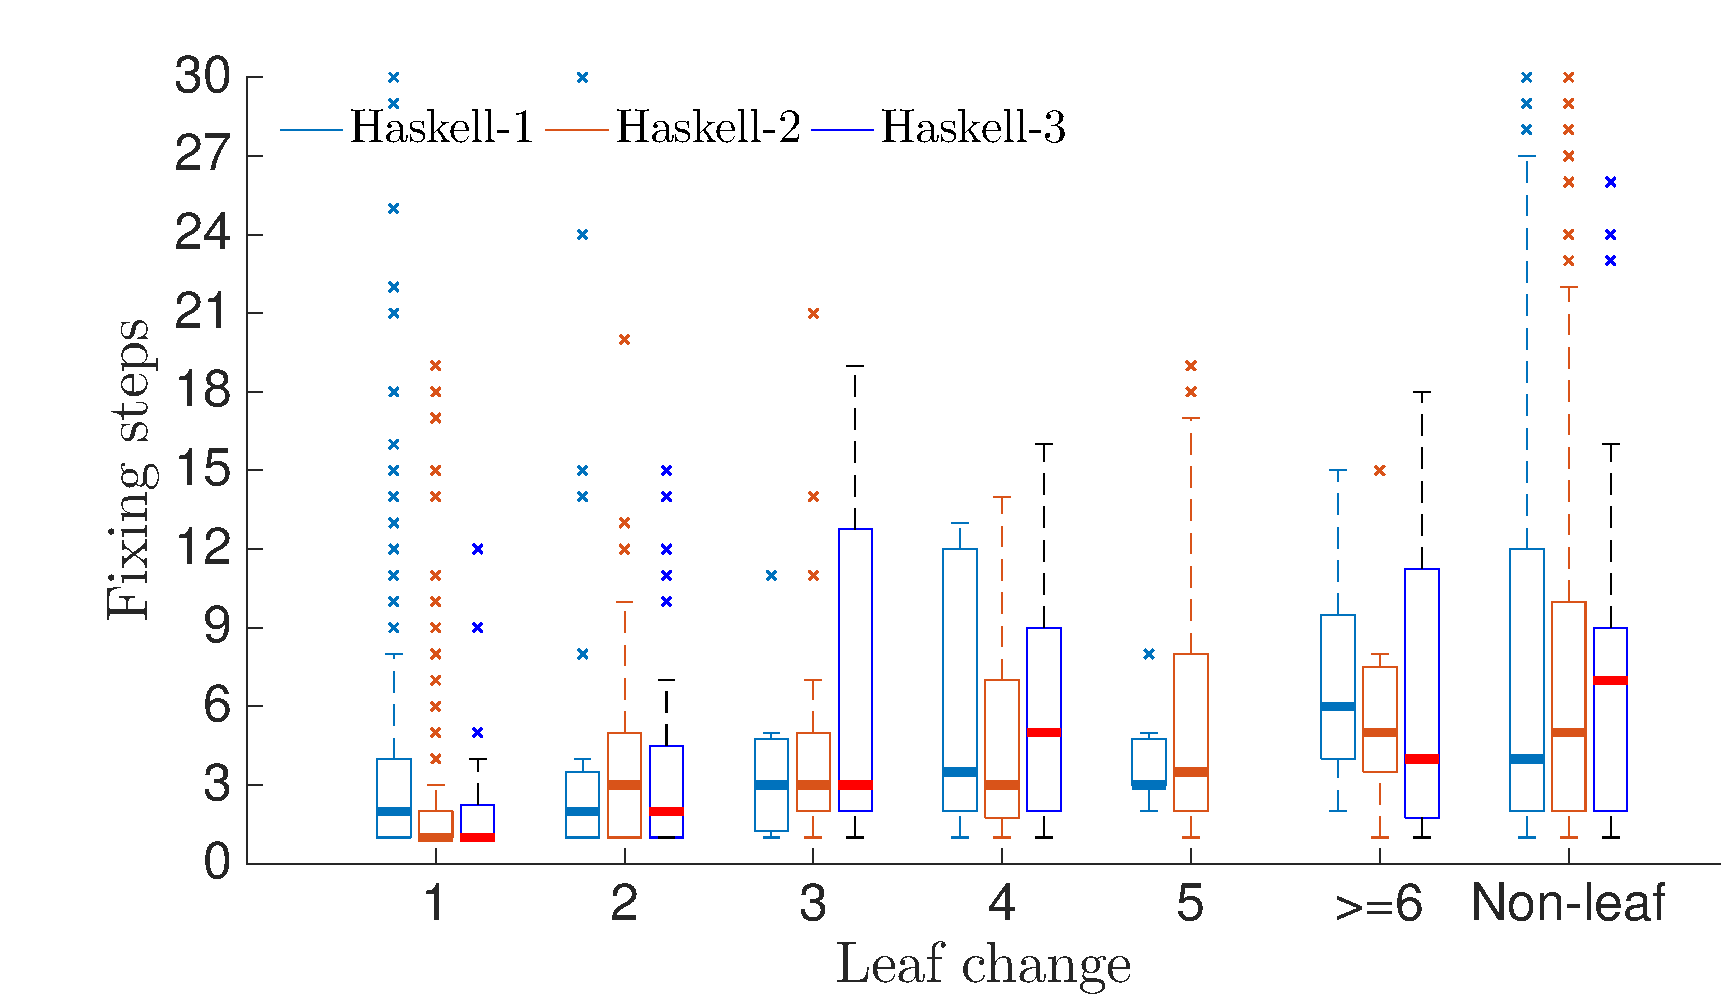
\includegraphics[width=1\columnwidth]{images/leaf_step-eps-converted-to.pdf}
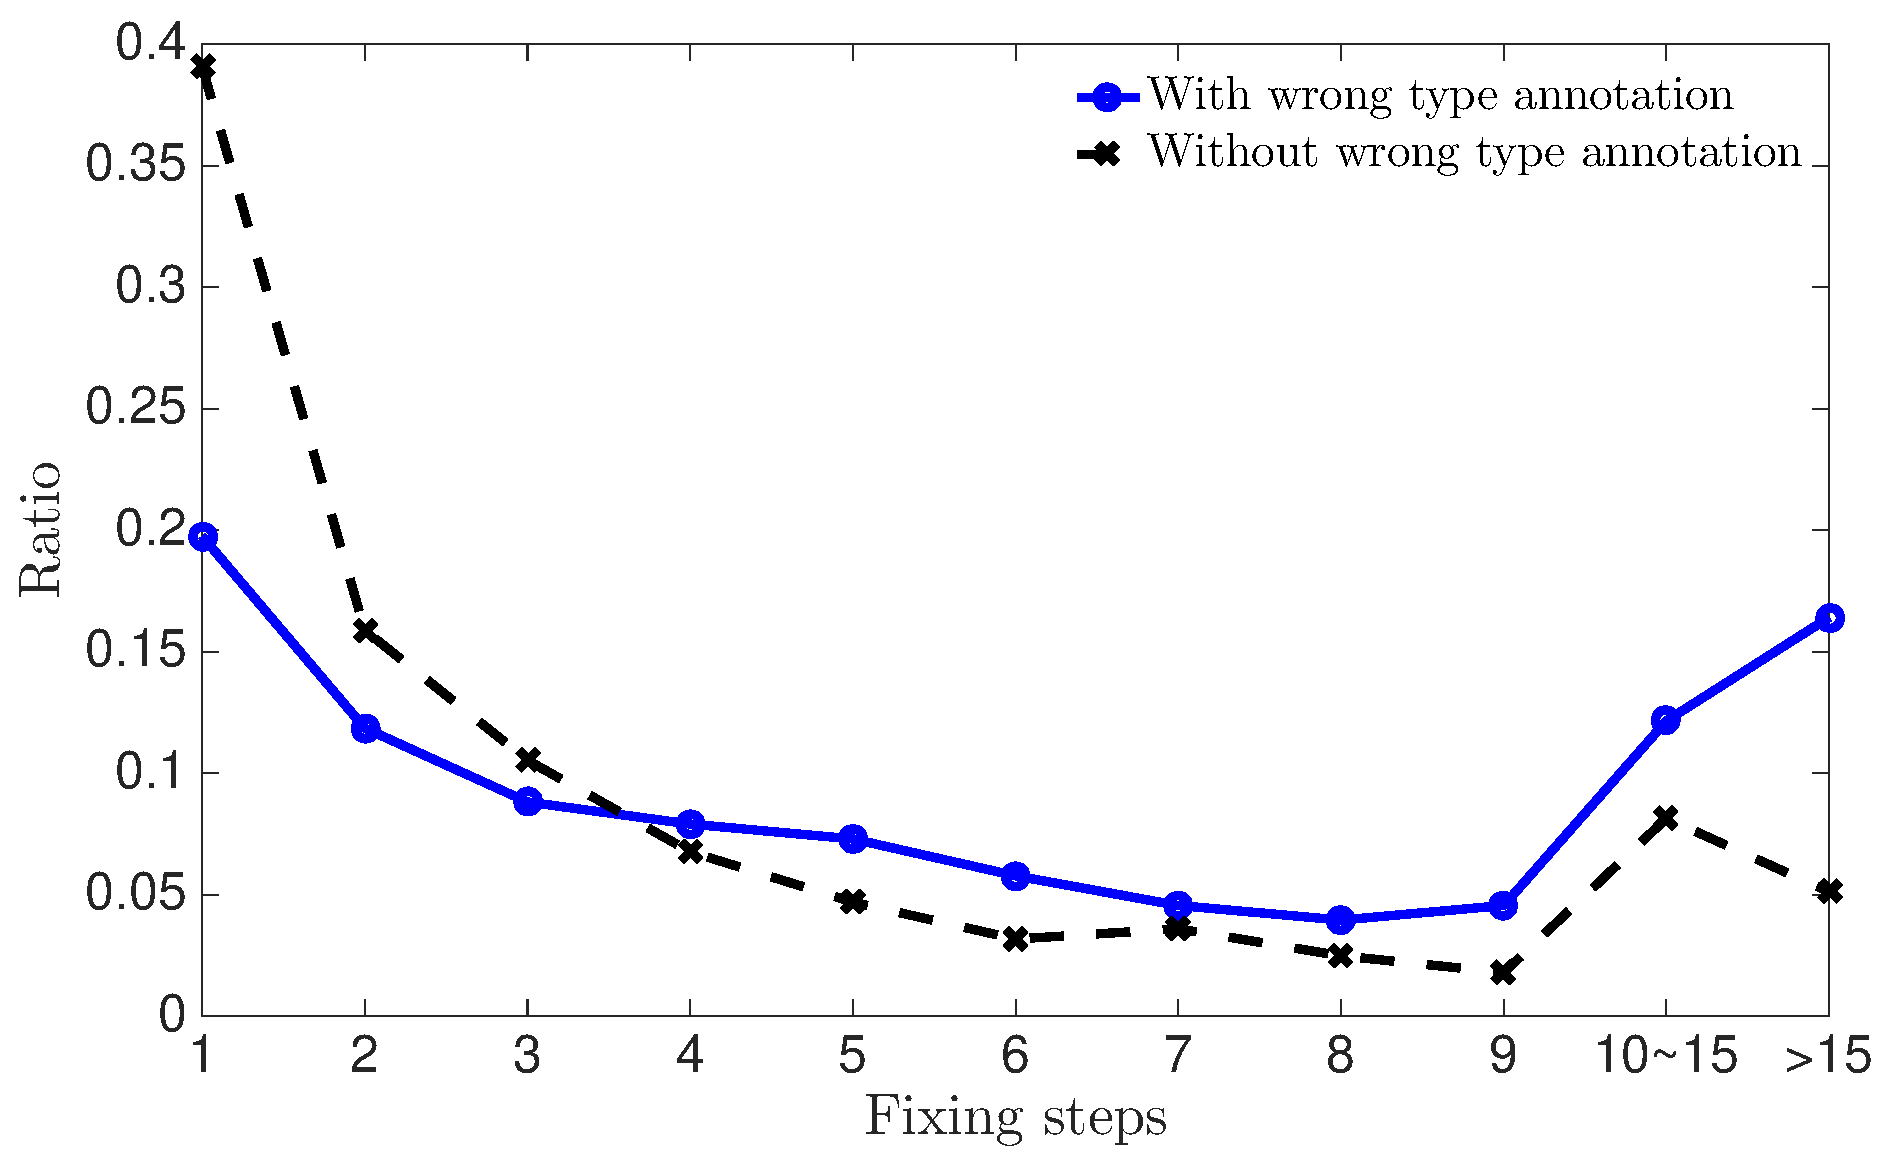
\includegraphics[width=.85\columnwidth]{images/wtn_comp.eps}
\caption{Effect of wrong type annotation on fixing steps}
\label{fig:wtn}
\end{figure}

Next, we study whether the presence of wrong type annotations affects
type error debugging or not.
The average steps for fixing type errors with
wrong type annotations in \benchs\
is 8.1 (\std=8.7), which is greater than 5.1,
the average number of steps for fixing
all type errors according to Section~\ref{sec:overview}.
%
We had the similar results for \benchf\ and \benchl.
Therefore, in general, fixing type errors with wrong type annotations
is more challenging for students than fixing other errors.
%
Moreover, in Figure~\ref{fig:wtn}, we present the distribution of 
numbers of fixing
steps for type errors with and without
wrong type annotations by merging
all the three data sets.
%\benchf\ and \benchs. 
When the number of fixing steps is smaller than 4,
We observe that the ratio for correct type annotations
is higher than that for wrong type annotations. 
%
%\benchf\ and \benchs. 
However, this phenomenon is reversed when the number of 
fixing steps is larger than 4. 
%
For example, for type errors with correct type annotations,
39\% of them can be fixed with single steps
and about 13\% of them need more than 10 steps to fix.
In contrast, those numbers are 20\% and 29\% for the wrong
type annotation case, respectively.
%20\% of the type errors with wrong type annotations are fixed with 1 step,
%and about 29\% of them need more than 10 steps to fix.
%

These results above indicate that it is difficult
for students to fix type errors when
wrong type annotations are involved.
One reason could be that Helium cannot
generate informative messages when type annotations are wrong,
%
Consider, for example, the following student program.
%
\begin{program}
lengte :: [[a]] -> [Int]
lengte x = maximum (map (length.head) x)
\end{program}
%
Helium produces the following error message.
%
\begin{program}
(33,12): Type error in right-hand side
 expression       : maximum (map (length . head) x)
   type           : Int
   does not match : [Int]
\end{program}
%
This error message led the student to inspect
the expression \prog{maximum (map (length . head) x)}
at line 33. Later, the student indeed changed it.
However, the correct fix should change the type annotation
from \prog{[[a]]->[Int]} to \prog{Table->Int} at line 32,
which is far away from the location reported in the error message.


To sum up, type annotations are not reliable,
especially in the beginner programs.
In addition, the error messages related to wrong type annotations
could be ineffective or even misleading,
and debugging wrong type annotations is difficult to students.
Worse, wrong type annotations happen together quite often
with other type errors, making the 
detection of them particularly challenging.

\section{When Are Error Message Effective?}
\label{sec:effectiveness}

Error messages generated by different debuggers
or even the same debugger
contain different kinds of messages, where some messages are more
concrete than others. In general, there are four kinds
of messages with increasingly
concrete information: \typel, \typet, \typer, and \typee.
For example, both \toolS~\cite{Zhang14:tgd,Zhang15:DTE} and  \toolMin~\cite{Pavlinovic14:FMT,Pavlinovic15:PST} generate
the first kind of messages only, which contains
location and the constraint that fails to solve.
All CFT~\cite{CE14popl}, Seminal~\cite{Lerner07:STM}, and
Helium can generate the latter three kinds of messages.
Our goal in this
section is to find out if certain kind of messages are
more effective than other kinds for debugging type errors.
%
We use \benchf\ and \benchs, 
which used Helium as the underlying compiler,
to analyze the message effectiveness, but exclude
\benchl\ since GHC doesn't have all kinds of error messages mentioned above.


The \typet\ kind message reports the inferred type and expected type
for the erroneous subexpression, which are also contained in
\typer\ and \typee\ kinds of messages.
The error message for \prog{lengte}
in Section~\ref{sec:annotation} belongs to this kind. 
The \typer\ kind
message explains the type error in a short sentence, and
%
one such example is the message for \prog{maxLength} in
Section~\ref{sec:subject:metric}. Finally, the \typee\ kind message
%
contains direct information about how to change the program
source code. 
Helium generates such a message for the following student program,
where it suggests to change \prog{(++)} to \prog{(:)}.
%
\begin{program}
toFirst :: [Int] -> [Int]
toFirst (x:xs) = x ++ toFirst (xs)

(3,22): Type error in variable
 expression       : ++
   type           : [a] -> [a  ] -> [a  ]
   expected type  : Int -> [Int] -> [Int]
 probable fix     : use : instead
\end{program}

\noindent
To study the effectiveness of error messages,
we first define the notion of \emph{error situation}, which are three
digits representing:
\begin{enumerate*}[label=(\alph*)]
\item does Helium locate the real error cause correctly,
\item whether following Helium's change suggestion will bring
the current program to the reference program, and
\item the distance between the real error cause and the one reported
by Helium in terms of the number of identifiers.
\end{enumerate*}
%
We have presented them in Section~\ref{sec:subject:metric} but reproduced them
here for the readability purpose.
For example, ``001'' means that Helium failed to locate the real error cause,
and following the message will not bring the program to the reference,
and the location Helium reported is 1 identifier away from the
real error cause.
%
The introduction of error situations is not to evaluate
the quality of Helium's error messages,
but rather to understand how different kinds of messages
affect error debugging in practice.


\begin{figure}
\centering
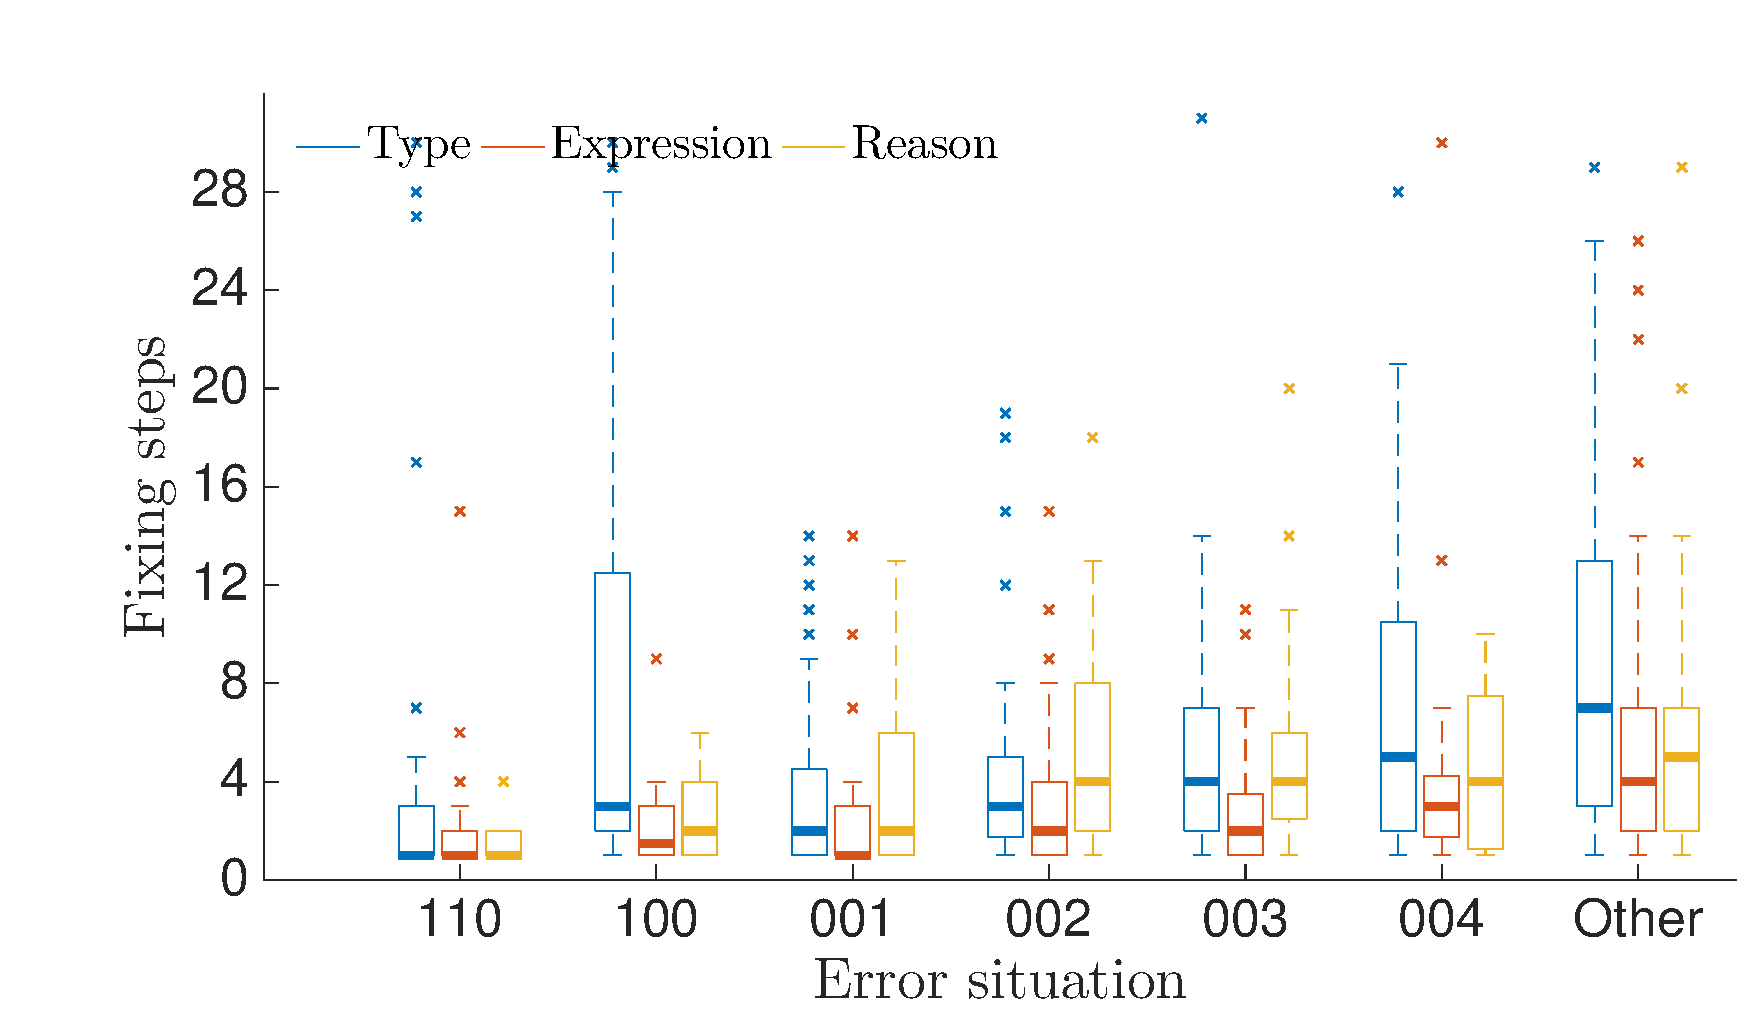
\includegraphics[width=0.85\columnwidth]{images/step_test.eps}
\caption{Error situation against fixing steps. The first digit
of each error situation denotes whether the message locates
the real error cause correctly (``1'') or not (``0''), the
second digit denotes whether following the message will bring
the corresponding program to the reference (``1'') or not (``0''), 
and the third digit measures the distance between the real error
cause and the location reported by Helium in terms of 
the number of identifiers.}
\label{fig:errsitu1}
\end{figure}

We can now classify each error message into one error situation
and further into one of the three kinds:
%For each error situation, we can classify a message into it.
%Furthermore, we classify a message based on one of the three message kinds, namely 
\typet, \typer, or \typee.
%
To measure the impact of error situations and message kind on
error debugging effectiveness, 
we use two metrics: the number of fixing steps and the size differences.
The number of fixing steps is calculated as, from the current programs,
how many steps are needed to reach the reference program.
%
An error situation with large number of fixing steps
indicates a hard debugging case.
%
We compute the size difference by comparing the next version of the current ill-typed program
and the reference.
A large size difference indicates that 
the program in the next step diverges to the reference,
and consequently students don't handle
the current error situation properly.

Figure~\ref{fig:errsitu1} shows the impact of 
different error situations and kinds of 
messages on fixing steps by merging \benchf\ 
and \benchs.
%
In general, we observe that
error situations and kinds of messages affect 
error debugging in the following aspects. First, 
as the reported location becomes further away from 
the real error cause, the number of fixing steps, 
for all message kinds, increases. 
%
The correlation coefficient between fixing steps and 
distances from the reported locations to real error causes
%with respect to the accuracy of error localization 
is 0.53 (\emph{p}-value=$1e^{-15}$). 
%
Second, 
%
the \typet\ kind error messages yields the largest
number of fixing steps for almost all error situations and
%
the \typee\ kind error messages yields the smallest
%number of fixing steps 
for any error situation.
%
%
More specifically, the average number of fixing steps
is 7.7 (\std=10.6) for the kind \typet, 
4.6 (\std=4.5) for the kind \typer, 
and 3.5 (\std=4.2) for the kind \typee.
%
The results show that, regardless of error situations,
type error debugging is less challenging to students when
error messages are more concrete. 

\begin{figure}
\centering
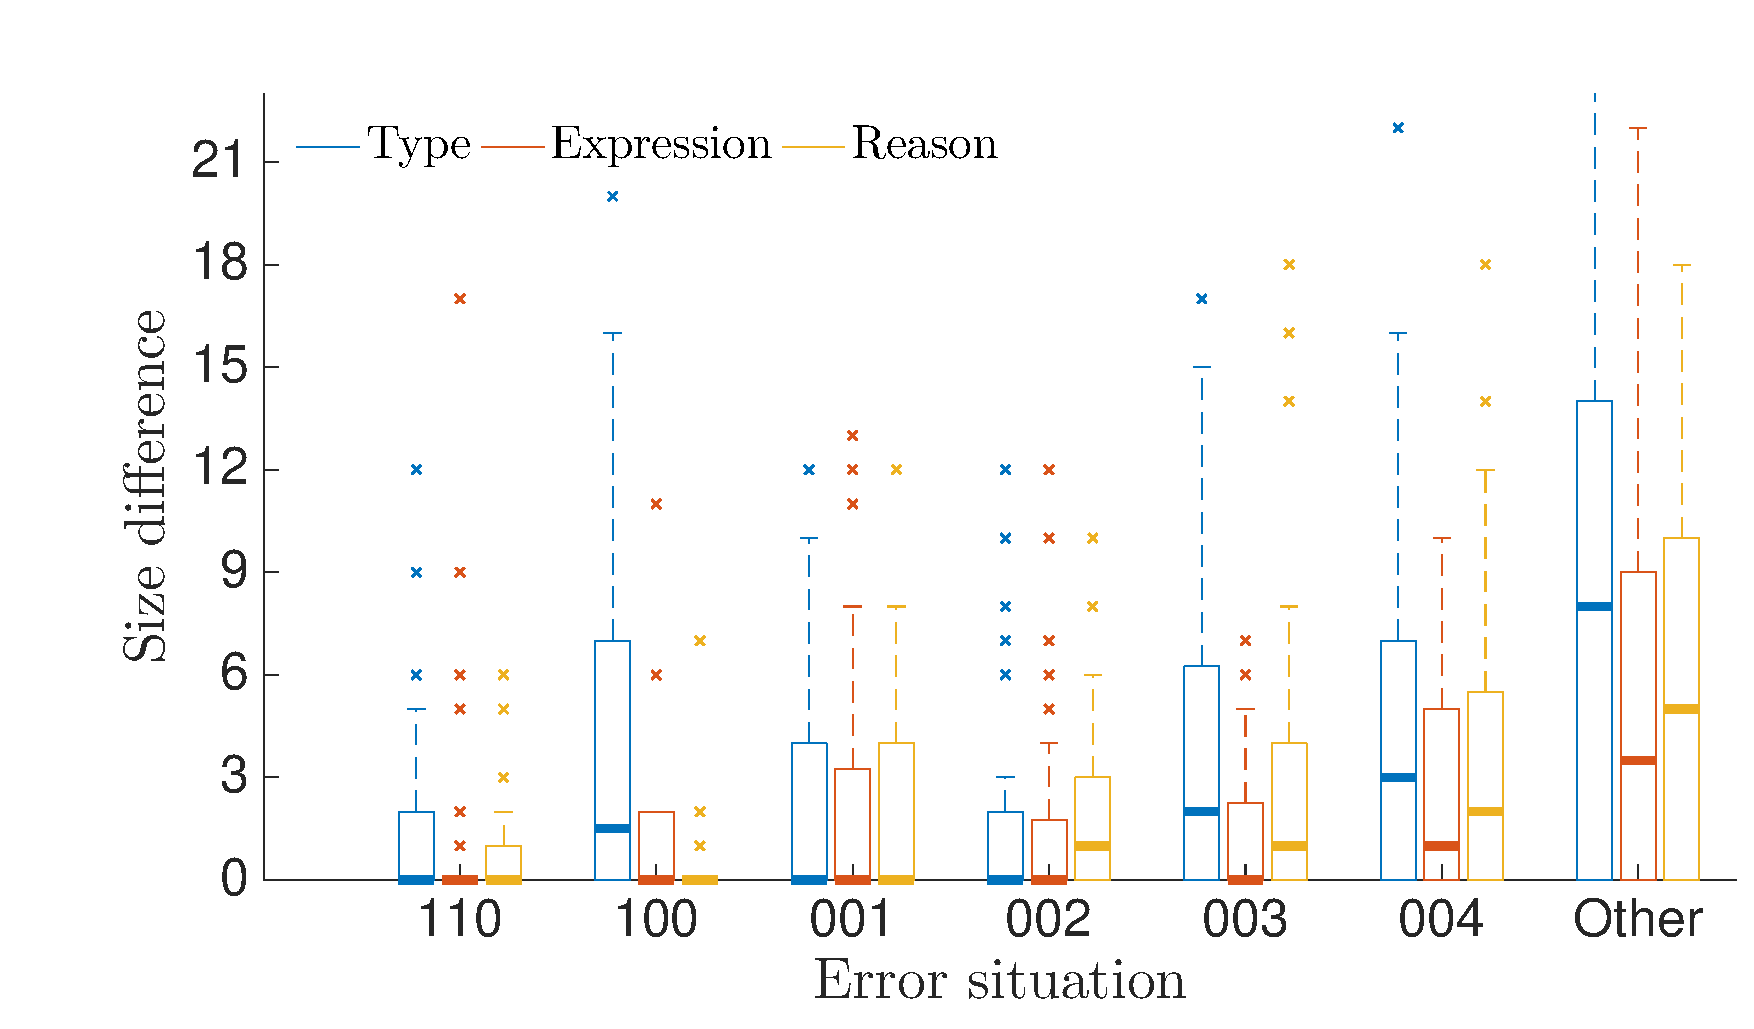
\includegraphics[width=0.85\columnwidth]{images/size_test.eps}
\caption{Error situation against size differences. The coding
scheme of error situations is the same as that 
in Figure~\ref{fig:errsitu1}.}
\label{fig:errsitu2}
\end{figure}

Figure~\ref{fig:errsitu2} shows the impact from
the perspective of size differences. We make similar 
observations from this figure as what we made from
Figure~\ref{fig:errsitu1}. 
%For example, the error
%situation ``110'' is most effective compared to
%other error situation. 
The size difference
becomes larger as the reported error location becomes
further away from the real error cause, with the
correlation coefficient being 0.48 (\emph{p}-value=$1e^{-15}$).
Moreover, within all error situations, the \typet\ kind
error message yields the largest size difference, with
an average of 5.6 (\std=6.4), while the average size differences
for the kinds \typer\ and \typer\ are 
4.1 (\std=5.5) and 2.7 (\std=4.9), respectively.
%
These numbers imply that more concrete and precise messages
are more useful for students to fix type errors.

\begin{figure}
\centering
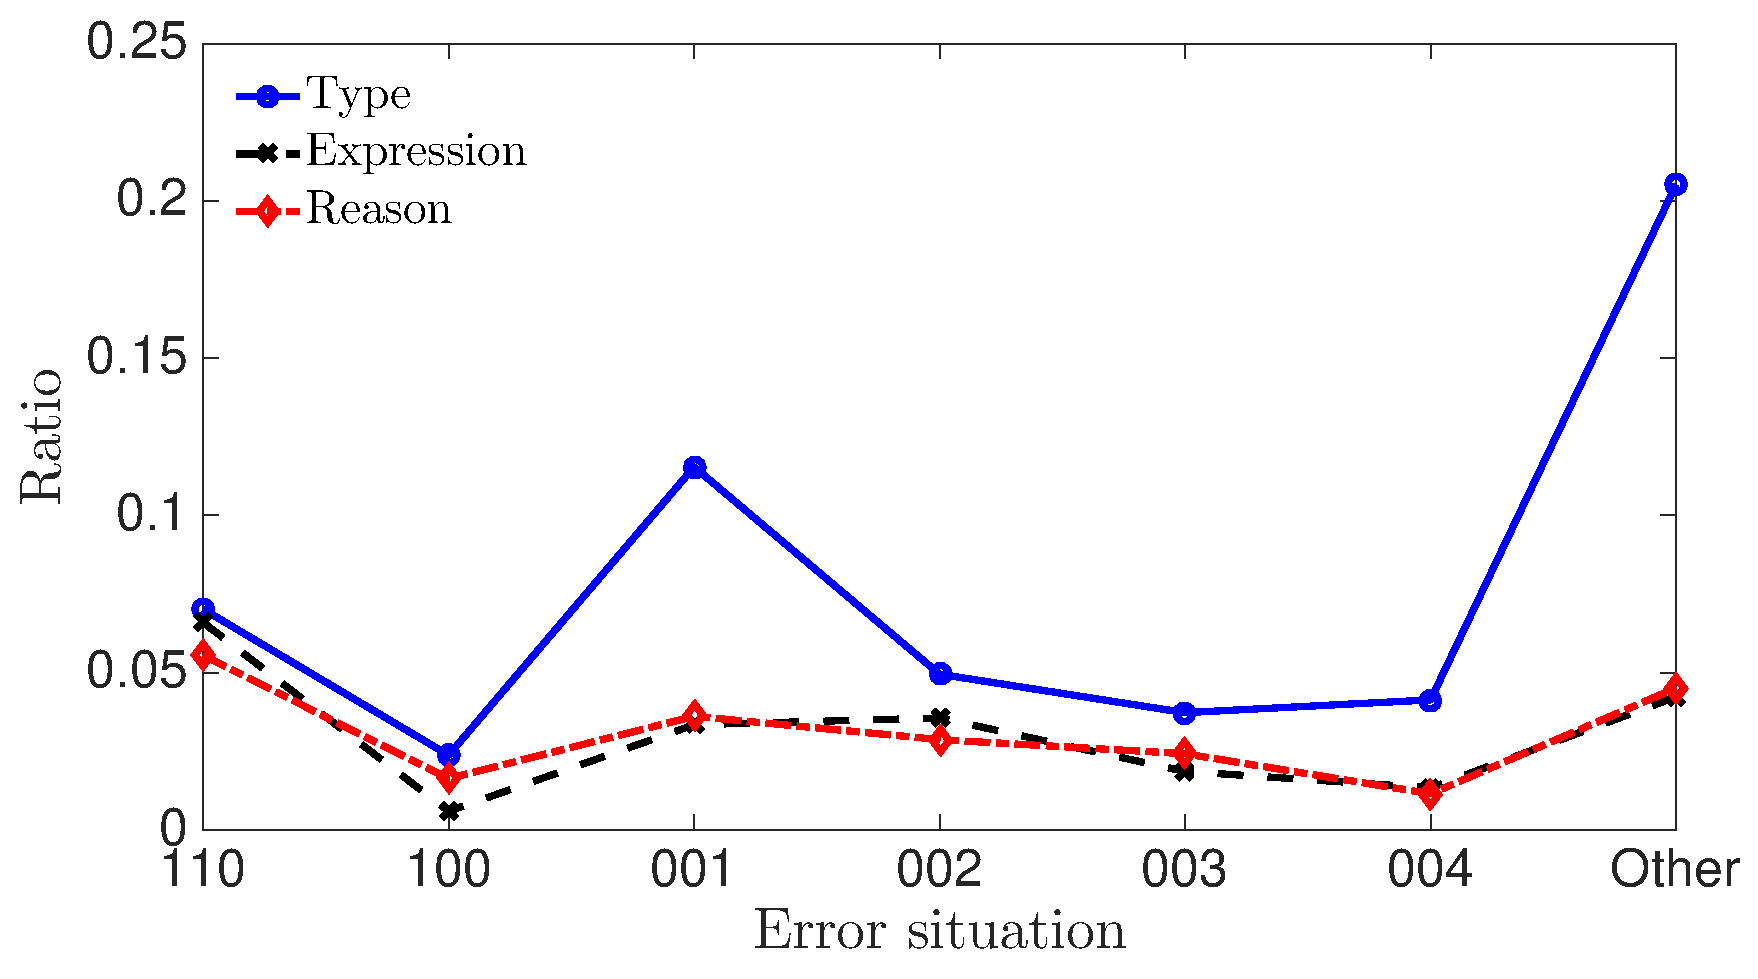
\includegraphics[width=0.85\columnwidth]{images/error_ratio.eps}
\caption{Distribution of error situation}
\label{fig:er}
\end{figure}

Error situations like ``110'' (correct error location and change suggestion)
or ``001'' (1 identifier away from the real error cause) are ideal,
since the number of fixing steps and size differences 
are both relatively small. 
Unfortunately, such situations happen rarely.
Figure~\ref{fig:er} presents the ratios of different situations that
students encountered during debugging type errors,
combining \benchf\ and \benchs\ together.
The ratio for the ideal situation, which we require
the median value 
of fixing steps to be smaller than 4 and that of size differences
to be smaller than 3, is below 10\%, close
to 5\% usually.
Worse,
the \typet\ kind messages appear most often in
all the error situations,
and the ratio is 0.21 in the situation where
the reported location is more than 4 identifiers away
from the real error cause.
This means that the prevalence of less concrete
error messages (the \typet\ kind) in hard debugging
situations (distance larger than 4) exacerbates
the challenges of fixing type errors for students.

We have done the same analysis by considering individual
weeks and have observed similar results. We omit the
details here. The results in this section suggest
that making messages more concrete or 
improving the accuracy of reported error locations
can help debug type errors, especially for novice programmers.

\section{What Language Features Are Difficult?}
\label{sec:difficulty}

In Section~\ref{sec:overview}, we have seen that
the average number of fixing steps in the program data sets 
is around 5.
In this section, we thus
consider type errors that require 
more than 5 steps to fix
as difficult.
%
To study if certain language features are correlated with the
difficulties that students encountered, 
we filtered out all the difficult errors in \benchf, \benchs, and
\benchl, which account for 30.6\% of all errors.
%
For each such error, we manually assign, when appropriate, one
or more difficulty reasons.


We give the meaning of each reason and 
describe how different reasons are assigned 
to a type error in Section~\ref{sec:diffr:reason}, 
where we also justify the selection of each difficulty reason.
Section~\ref{sec:diffr:res} shows some statistical results 
and the impacts of difficulty reasons.
We hope our findings could be exploited
for developing future error debuggers
or could be used to organize course materials
more appropriately.

\begin{figure}
\centering
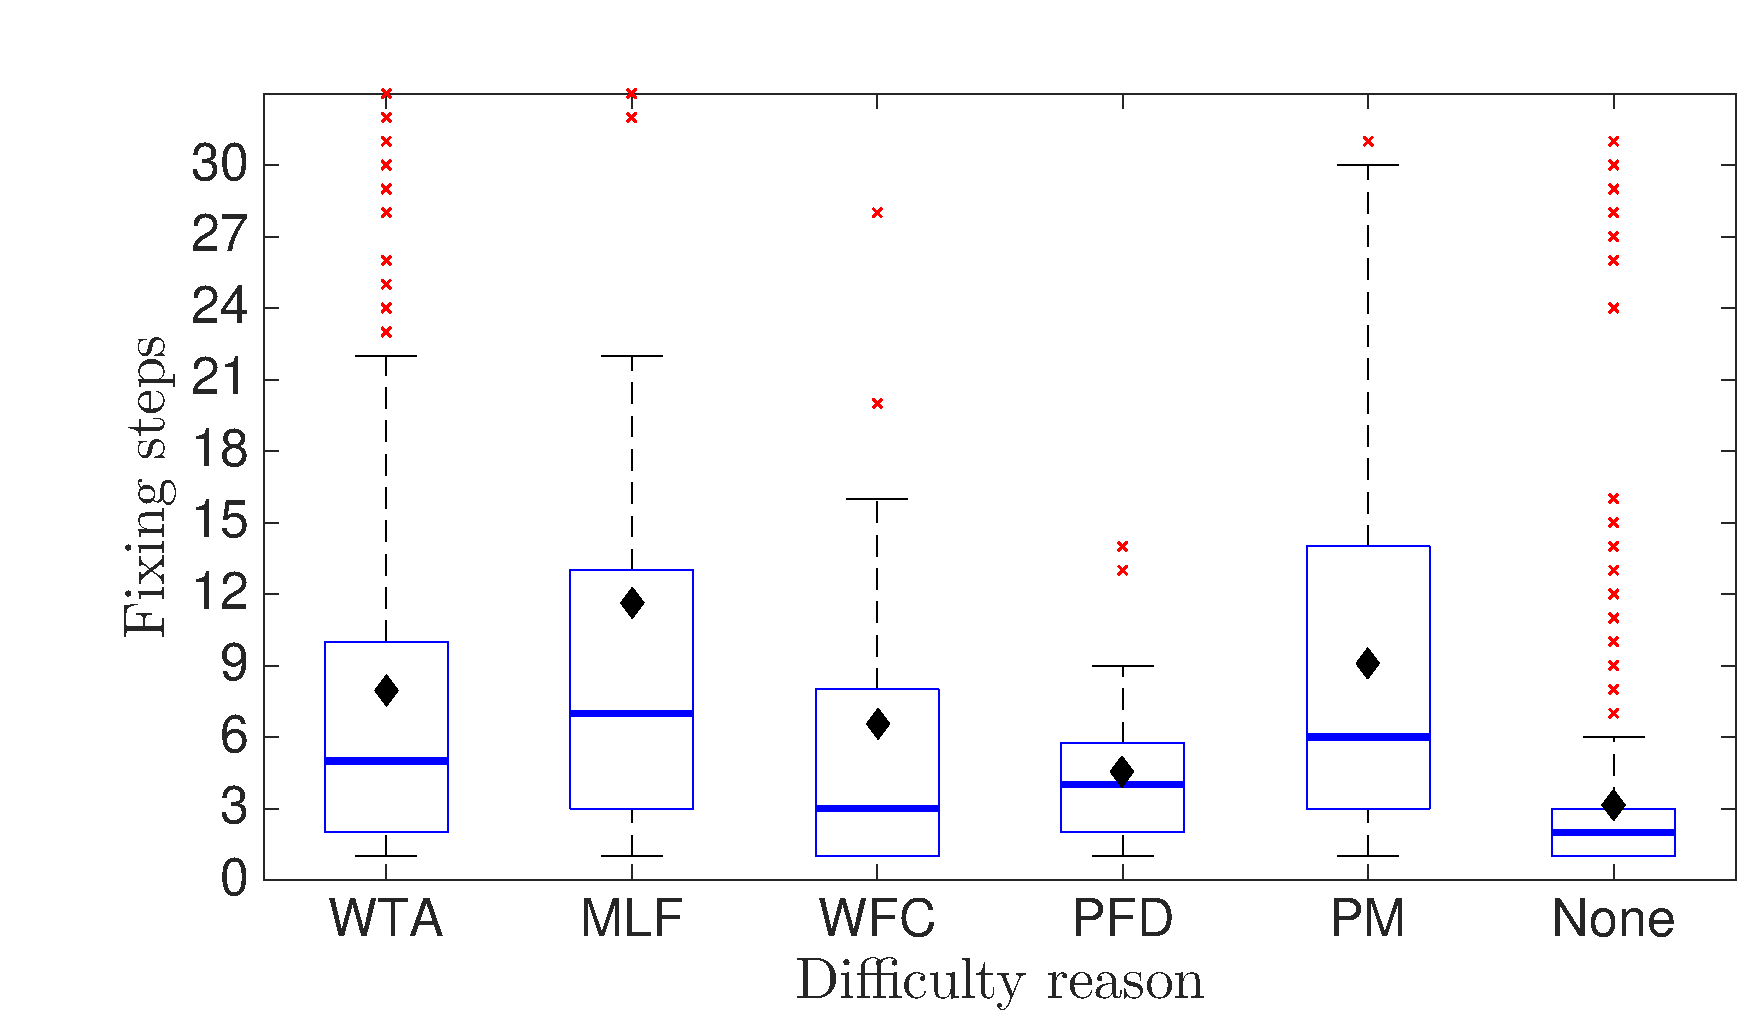
\includegraphics[width=0.85\columnwidth]{images/step_diffr.eps}
\caption{Difficulty reason against fixing steps.
The figure considers all type errors that have the corresponding
difficulty reason, including those that
were fixed within 5 steps.
%
We use a black diamond to represent the average number of steps for each reason.
The average number of fixing steps for all type errors is 5.1 (\std=6.6).
We use the acronyms ``WTA'', ``MLF'', ``WFC'', ``PFD'' and ``PM'' to represent \emph{wrong type annotation}, \emph{multiple library functions}, \emph{wrong function composition}, \emph{point-free function definition}, and \emph{pattern matching}, respectively. ``None'' denotes the errors without assigning any difficulty reason.}
\label{fig:diffr2}
\end{figure}


\subsection{Meanings of difficulty reasons}
\label{sec:diffr:reason}

We found out five main difficulty reasons
that students struggled
when debugging type errors. We identify these
difficulty reasons by comparing the ill-typed
program with the reference program. 
We discuss each difficulty reason below.

\paragraph{Wrong type annotation}
%
We have shown that type annotations are
unreliable and
fixing wrong type annotations usually
needs more effort in Section~\ref{sec:annotation}.
%
%
For example, in the following function
\prog{getTable}, the type error was fixed
by changing the type annotation from
\prog{Table -> String} to
\prog{[String] -> String}, and it
took the student 16 steps to fix. Since only the
type annotation in the ill-typed program is changed in the reference program,
%are the only difference between
%the ill-typed program and the reference program,
we assign ``wrong type annotation'' as the difficult
reason for fixing this type error.
\begin{program}
getTable :: Table -> String
getTable [] = []
getTable (x:xs) = (x ++ "\textbackslash{n}") ++ getTable xs
\it{getTable :: [String] -> String}
\end{program}
%
%
Note that
%, among all type errors including the difficult ones, 
some type errors that are caused
by wrong type annotations can be fixed within 5 steps. 
%Note we can assign this reason to type errors that are fixed
%within 5 steps. 
As a result, it would be interesting to 
know whether this is a real difficulty reason in general.
To address this question, we gathered all the type errors
that were caused by wrong type annotations and investigated
the fixing steps for such errors.
%
Figure~\ref{fig:diffr2} shows that, 
in average, the number of steps to fix these type errors
are 7.9 (\std=8.7), which is larger than that to fix
all type errors.
Therefore, ``wrong type annotations'' is a real difficulty
in fixing type errors. 

\paragraph{Involvement of more than two library functions}
%
When an expression contains more than two library functions,
it usually becomes long and relatively complex.
Since beginners are not very familiar with the types of library functions,
it could be a problem for them to infer whether the whole expression
involving multiple library functions is type correct or not.
%
%
Take the following function \prog{writeLine} as an example, which took
the student 6 steps to fix.
We view that the involvement of multiple library function
as the difficult reason in this example because the use of library functions
\prog{repeat} and \prog{take} complicates the type reasoning,
although the type error is fixed by just changing \progdq{-}
to \progsq{-}.
%
\begin{program}
writeLine :: [Int] -> String
writeLine []     = ""
writeLine (x:xs) = '+' : take x (repeat "-") : writeLine xs
\it{writeLine (x:xs) = '+' : take x (repeat '-') ++ writeLine xs}
\end{program}
%
In Figure~\ref{fig:diffr2}, we present the average number
of steps to fix the type errors caused by this difficulty. 
In average, fixing these type errors took 11.6 (\std=13.1)
steps, which is much greater than
the fixing steps for all type errors. 
Therefore, this
difficulty poses real challenges to error debugging in practice.

\paragraph{Wrong function composition}
%
We observed that type errors are very likely to happen
when \prog{\$}, \prog{(.)}, partial applications,
and parentheses and brackets are used together,
since students do not have good understandings of
associativity and precedence. 
%
In the following example, 
the number of steps to fix the type error in the function \prog{insertionSort} 
is 15.
This error, caused by the mistake of function composition,
is fixed by adding a pair of parentheses around the last
two subexpressions in the body.
%
\begin{program}
insert :: Int -> [Int] -> [Int]
insertionSort :: [Int] -> [Int]
insertionSort lijst = insert (head lijst) insertionSort (tail lijst)
\it{insertionSort lijst = insert (head lijst) (insertionSort (tail lijst))}
\end{program}
%
In average, all type errors assigned with this difficulty reason
took 6.5 (\std=8.7) steps to fix, greater than the 
steps for fixing all type errors. Thus, this is a
real difficulty in fixing type errors. 

\paragraph{Point-free function definition}
%
Point-free functions
help to write compact and clear code. It is
also recommended writing function definitions in
this style when possible.
However, as this style is quite different
from imperative languages that many students are familiar
with, they may take time to get used to it.
We found out that in most cases students changed back
to pointful function definitions
when type errors are related to point-free function definitions.
%In addition, point-free style makes error
%debugging become harder for higher-order functions.
The type error in the function \prog{afterFirst} below
is fixed by adding the parameter to the function definition,
and it took the student 6 steps to fix. Since only the 
function parameter style is changed in the reference program,
we assign ``point-free definition'' as the difficulty reason in this example.
%
\begin{program}
afterFirst :: [Int] -> [Int]
afterFirst = tail \$ dropWhile (/=0)
\it{afterFirst xs = tail \$ dropWhile (/=0) xs}
\end{program}
%
The average number of 
steps students took to fix type errors assigned this difficult
reason is 4.8 (\std=3.4), slightly smaller than
the average number of steps for fixing all type errors. 
%even a little smaller than that average value for all type errors.
However, we still view point-free function definition as one 
difficulty reason because students usually fixed such errors
by ``avoiding'' them rather than by ``overcoming'' them. Specifically,
students fixed such errors by adding parameters to the point-free function definition 
and making corresponding changes in the function body.
%used a workaround to fix this kind of errors
%by using pointful function definitions instead.

\paragraph{Pattern matching}
%
Pattern matching is one of the basic features in
functional programming. Errors in patterns usually
lead to inaccurate and non-informative error 
messages. 
We use the following example
from student program data sets
to show why type errors caused by pattern matching
are hard to fix.
%
\begin{program}
serialization :: [[a]] -> [a]
serialization [h:t] = h ++ serialization t
\it{serialization (h:t) = h ++ serialization t}
\end{program}
%
The error message generated by Helium is:
%
\begin{program}
(6,19): Type error in right-hand side
 expression       : h ++ serialization t
   type           : [a  ]
   does not match : [[a]]
 because          : unification would give infinite type
\end{program}
%
This message fails to locate the real error cause and
conveys the type error in compiler jargon, making
error debugging particularly difficult for students. 
As a result, the type 
error in \prog{serialization} took the student 18 steps to fix. 
%
In Figure~\ref{fig:diffr2}, we present the average number
of steps for fixing type errors that are assigned this difficulty. 
In average, such type errors took 
9.1 (\std=7.9) steps to fix, much more than the steps to fix all type errors.
Therefore, ``pattern matching'' is a
real difficulty in fixing type errors. 

In some cases, we assign multiple difficulty reasons
to a single type error. 
For example, for the type error in the following
function \prog{removeFstColumn}, 
we assign three difficulty reasons (``wrong type
annotation'', ``multiple library functions'',
and ``wrong function composition'') since all of them apply
here. This error took the student 13 steps to fix.
%
%
\begin{program}
removeFstColumn :: Table -> String
removeFstColumn t = transpose.tail (transpose t)
\it{removeFstColumn :: Table -> Table}
\it{removeFstColumn t = transpose (tail (transpose t))}
\end{program}
%

In very few cases, the type errors were obvious to fix 
but still took the student more than 5 steps to fix. We did
not assign any difficulty reason for these cases.
%
For example, the type error in the function \prog{seperator} below is such a case,
which took
the student 6 steps to fix. 
Helium exactly suggests
to change \progdq{-} to \progsq{-} to fix the type error,
but the student 
was maybe not careful enough when debugging the error.
%
\begin{program}
seperator :: [Int] -> String
seperator [] = []
seperator (x:xs) = replicate x "-" ++ seperator xs
\it{seperator (x:xs) = replicate x '-' ++ seperator xs}
\end{program}
%
In other cases that a type error was fixed by rewritting the majority
of the program, we did not assign any difficulty reason either.
%
%
For the type errors we did not assign any
difficulty reason, they took, in average, 
3.1 (\std=4.5) steps to fix. This value is much smaller
than the average number of step for fixing all type error,
suggesting that those errors that are not covered by the five difficulty reasons
will not affect our analysis on the difficulties in fixing type error much.


\subsection{Impacts of difficulty reasons}
\label{sec:diffr:res}

Figure~\ref{fig:diffr1} shows
the distribution of these reasons, where
each ratio is computed as the number of
errors that are difficult
for the corresponding reason over the type errors that took more than
5 steps to fix. All the ratios in the figure do not
sum up to 1 because some errors are assigned multiple
difficulty reasons.
%
It would be meaningful to show how the ratios of
difficulty reasons evolve over the time.
However, 
%since we only considered these difficult
%type errors (the number of fixing steps is bigger than 5),
some weeks do not have enough data for us to perform 
a statistical analysis.

\begin{figure}
\centering
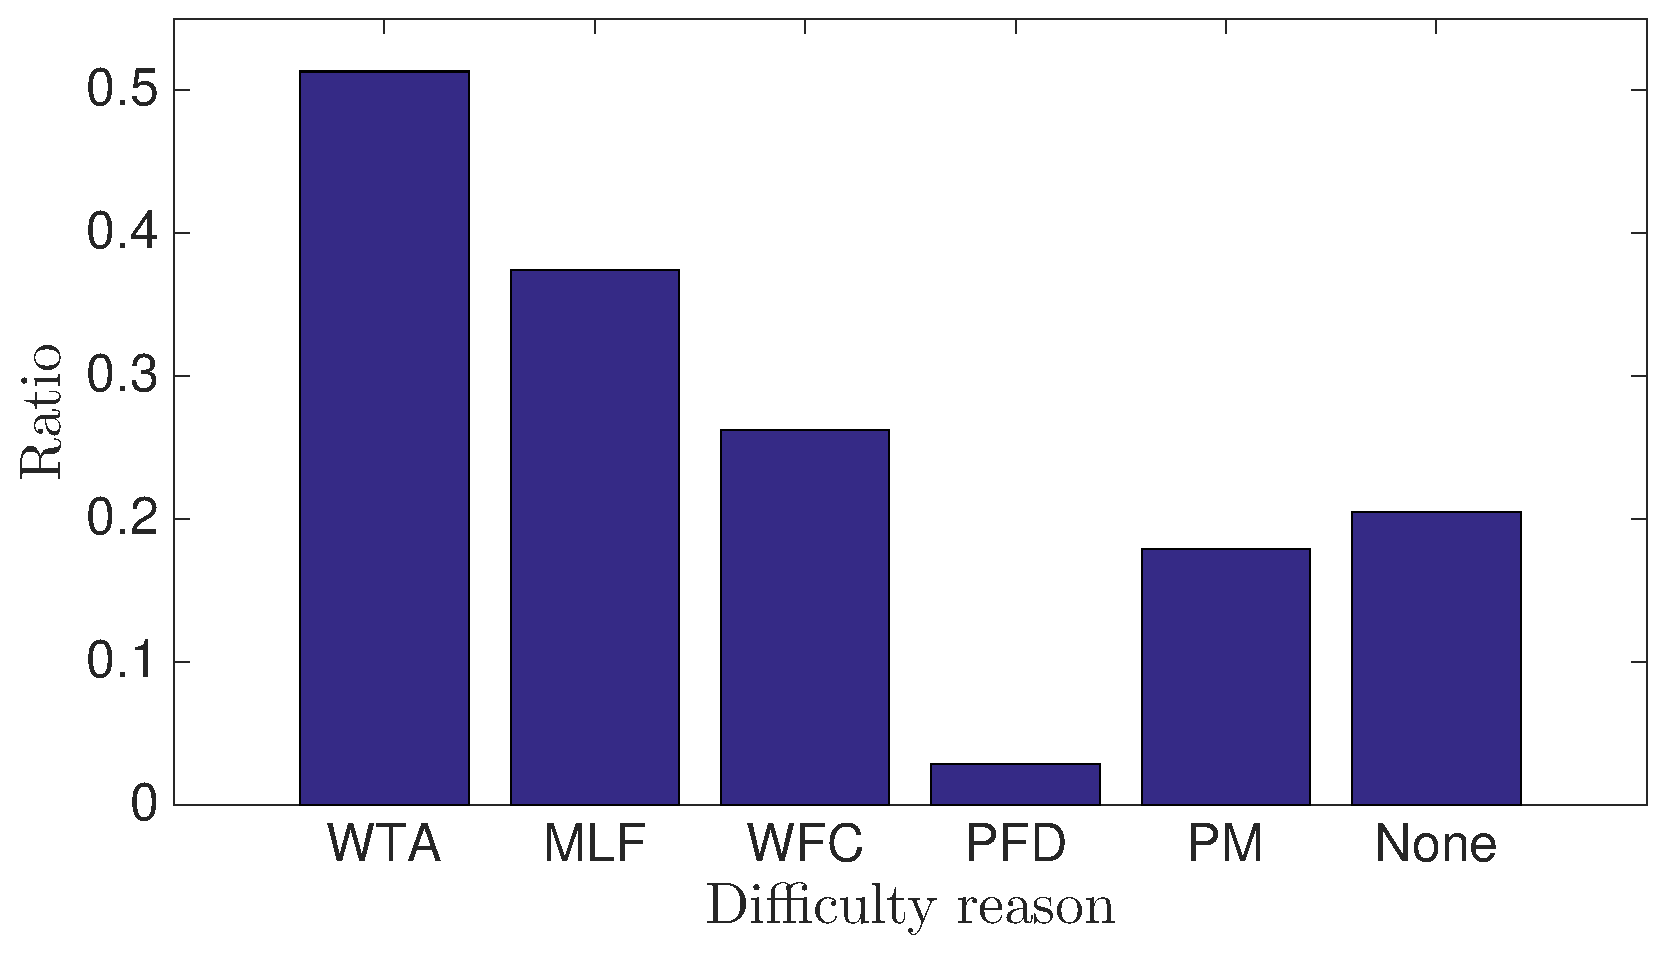
\includegraphics[width=0.85\columnwidth]{images/diffr.eps}
\caption{Distribution of difficulty reasons. The figure considers
all type errors that are fixed with more than 5 steps. The labels on 
the x-axis have the same meanings as those in Figure~\ref{fig:diffr2}.
}
\label{fig:diffr1}
\end{figure}


The ratio that students
encountered wrong type annotations as
the difficult reason
is the highest (more than 50\%) among all difficulties.
Unfortunately, we noticed that few 
approaches~\cite{chen2014let} tried
to locate wrong type annotations.
The result indicates that students should check
the correctness of type annotations when they encounter type errors.

About 37\% of the difficult errors are related 
to more than two library functions.
Moreover, we found out that such errors are often assigned
other reasons too, which increases the difficulty in debugging them.
For example, multiple library functions as well as
wrong type annotation and wrong function composition
contribute to the difficulty of fixing
the type error in \prog{removeFstColumn}.
As a result, the average number of fixing steps
for this difficulty reason is the largest in Figure~\ref{fig:diffr2}.
This result suggests that error explanation 
methods~\cite{Chitil01:CET}
could be useful to novice programmers
when debugging this kind of difficult errors.

Wrong function composition accounted for
about 26\% of all difficult type errors.
Note that most error debuggers do not work well
for such errors since they are usually fixed
by adding or removing pairs of parentheses. 
%As shown in Figure~\ref{fig:lst}, such type errors
%take more steps to fix.
From the educational view,
while functional programming languages provide
good flexibility for composing functions,
students might
better defer using them but write nested expressions
with parentheses 
when they first started to learn 
functional programming.

Point-free definitions accounted for 
less than 5\% of difficult type errors.
%
%There are not many type errors (less than 5\%) 
%that are caused by point-free function definition.
This is because students did not use such style
very often. However, as mentioned in 
Section~\ref{sec:diffr:reason}, whenever students
encountered errors with this difficulty, they adopted a workaround to fix
such errors by adding parameters to function
definitions. 
%
Another observation we had while investigating
students programs was that students used point-free
style definitions rarely in their well-typed
parts of programs. 
%
All these findings together imply that students probably did not
comprehend this language feature well.
%We recommend that instructors defer teaching this
%until the students have become proficient with the language.

Pattern matching accounted for about 17\% of all difficult
errors. 
%The ratio of pattern matching errors is only about 17\%,
%which means not many difficult errors belong to this kind.
%However, 
Figure~\ref{fig:diffr2} shows that the average number of steps 
to fix these type errors is the second largest among 
all difficulty reasons.
Mainly this is because that
the generated messages for pattern matching errors
are usually not informative, or even misleading.
To ease the difficulty of debugging such errors,
it is important for students to understand 
correct uses of patterns.

\section{Threats to Validity}
\label{sec:threat}

There are many potential threats to the validity of our study.
First, we have considered only three data sets. Increasing the
number of data sets always increases the validity
of a study. However, due to the particular aspects we are
investigating, many data sets available through git
repositories or Massive Online Open Courses don't
suit our needs. Such data sets contain only final
versions of programs, which are either well-typed or
while ill-typed but we don't have information about
how the type errors should be fixed. Also,
some data set is inaccessible to us due to
permission reasons~\cite{tirronen2015understanding}.
Nevertheless, we have gathered most data sets
available in the research community that suit
our needs. Fortunately, these data sets were written 
%in different languages and 
by different programmers,
used different compilers, and program sizes are quite
diverse, from several lines to several hundred lines.
While two data sets \benchf\ and \benchs\ were collected
at the same university, the programming assignments
were quite different, for example, some assignments
were present in one year while absent in the other year.
For these reasons, we believe that our data sets are quite
representative. Nevertheless, considering
more data sets will give a broader view of error debugging
in practice.


Second, the analysis of fixing process may be affected
by the compiler the students were using. This paper
contains two main kinds of analysis, the final fix and the
fixing process. Since the final fix analysis
considered only the ill-typed programs and the final fixed
programs, the result should not be affected by the compiler
being used. The fixing process considered two consecutive
versions by the student, and the second version may
be directed by the error message from the compiler that
was used. However, this issue seems hard to avoid since the
error message has to be generated by some compiler or
error debugger anyways. Moreover, from Figure~\ref{fig:lst},
we observed that the results of using GHC and Helium are
similar. For this reason, we believe that the compilers being
used should pose few threats.


Finally, the majority of the study is performed by
a single student. Processing all ill-typed programs
manually is very time consuming.
%, it takes the person
%about 600 hours to finish.
It's hard to allocate
another student to repeat the same work.
We took 
several approaches to minimize the potential biases that
may be introduced.
First, in the beginning, two persons processed
same programs and the results were discussed to
reach agreement. Second, while inspecting
the programs, one person first went through
the whole program sequences to fully understand
users' intention and then analyze each program.
This helped to choose correct reference programs.

\chapter{Nonstructural Type Error Representation}
\label{sec:features}

\section{Unifying Non-Unifiable Types}
\label{sec:features:unify}

\section{The Feature Vector}
\label{sec:features:feature}

\chapter{Learning Nonstructural Errors -- \newCompiler}
\label{sec:solution}

\section{Motivation for Using Machine Learning}
\label{sec:solution:motivation}

\section{The Proposed Approach}
\label{sec:solution:approach}

\subsection{Preliminaries of Machine Learning}

\subsection{Data Preprocessing}

\subsection{Imbalanced Classification}

\subsection{Implementation}

\section{Evaluation}
\label{sec:solution:eval}


\chapter{Conclusion and Future Work}
\label{sec:conclusion}

\section{Other Applications}
\label{sec:conclusion:other}

\section{Main Contributions and Future Directions}
\label{sec:conclusion:close}

%\include{chapter11}	

%\include{chapter12}	
%
% Appendix/Appendices
%
% If you have only one appendix, use the command \appendix instead
% of \appendices.
%
%\appendices

%\include{chapter-appendix1}
%\include{chapter-appendix2}
%\include{chapter-appendix3}

%
% Generate the bibliography.
%

%\nocite{*}      % This command causes all items in the               %
                % bibliographic database to be added to              %
                % the bibliography, even if they are not             %
                % explicitly cited in the text.                      %

% Here the bibliography is inserted.
% Replace "example" with the name of your ".bib" file
\bibliography{error-reporting,me,paper,pldi}                      
\index{Bibliography@\emph{Bibliography}}
%


%
% Generate the index.
% 
%
\printindex     % Include the index here. Comment out this line      
%               % with a percent sign if you do not want an index .  
%

\begin{abstract}
test
\end{abstract}

\end{document}
% The following comment block is used by the different flavors of EMACS and
% the AUCTEX package to manage multiple documents.  In order for AUCTEX
% to understand you're working with multiple files, you should define
% the TeX-master variable as a file local variable that identifies your
% master document.
%
% Please do not remove.
%%% Local Variables: 
%%% mode: latex
%%% TeX-master: "example.tex"
%%% End: 
